\documentclass[
    corpo=12pt,
    oneside,
    evenboxes,
    tipotesi=triennale,
    stile=classica,
    oldstyle,
    autoretitolo,
    greek,
]{toptesi}
\usepackage[utf8]{inputenc}
\usepackage[T1]{fontenc}
\usepackage{lmodern}
\usepackage{hyperref}
\usepackage{setspace}
\usepackage{verbatim}
\usepackage{pgfplots}
\usepackage{graphicx}
\usepackage{subfig}
\usepackage{amsmath}
\usepackage{eurosym}
\usepackage{enumerate}
\usepackage{booktabs}
\usepackage{tabularx}
\onehalfspacing

\hypersetup{
    pdfpagemode={UseOutlines},
    bookmarksopen,
    pdfstartview={FitH},
    colorlinks,
    linkcolor={blue},
    citecolor={blue},
    urlcolor={blue}
  }
\usepackage{lipsum}

\newtheorem{osservazione}{Osservazione}

\begin{document}\errorcontextlines=9

\begin{ThesisTitlePage}
    \ateneo{Universit\`a degli Studi di Torino}
    \StrutturaDi{Dipartimento di Management}
    \struttura[]{}
    \NomeElaborato{Tesi di laurea triennale}
    \titolo{Lo stato di salute del Calcio pre e post COVID-19}
    \sottotitolo{Fair Play Fiananziario e Superlega}     
    \corsodistudi{Management dell'Informazione e della Comunicazione Aziendale}
    \candidato{Riccardo \textsc{Borgo}}
    \relatore{prof.ssa ~Simona \textsc{Alfiero}}
    \sedutadilaurea{\textsc{Anno~accademico} 2021-2022}
    \logosede{img/Unito-logo, img/logo_saa.jpeg}
\end{ThesisTitlePage}

\figurespagetrue
\indici

\mainmatter
\begin{interlinea}{1.5}
    
\chapter{Introduzione generale}
Durante lo sviluppo di questa trattazione si andrà ad analizzare lo "stato di salute" del calcio europeo prima e dopo 
l'avvento della pandemia COVID19 che ha sicuramente stravolto la vita di tutti ed ha sicuramente arrecato non pochi danni 
economici al mondo, compreso quello del calcio.\newline
Il primo capitolo verter\'a principalmente sull'analisi della situazione economica pre-pandemia, per permettere di delineare una situazione
completa e capire se anche prima del 2020 esistessero gi\'a dei problemi nell'economia del calcio. Per primo verr\'a approfondito lo scenario
globale all'interno dei 5 pi\'u importanti Paesi Europei: Italia, Francia, Germania, Spagna e Inghilterra. Essi sono le realt\'a pi\'u 
affermate e potenti all'interno del sistema calcio, nonstante negli ultimi anni stiano crescendo molto anche altri campionati come per esempio
quello Olandese e altri dall'Est Europa. Questa prima parte avr\'a come argomento due indicatori principali: \textbf{Risultato Economico 2019} 
con la sua relativa scomposizione in \textbf{costi} e \textbf{ricavi} e gli \textbf{stipendi}. Questi due elementi
permettono di generare un'opinione trasversale e completa della situazione. Verrà mostrato come non in tutti 
si riesca ad arrivare ad un risultati positivo, andando quindi a rendere in qualche modo 
"unico" ogni campionato e la sua relativa Federazione. Le Federazioni (uniche per ogni Stato) hanno il compito
comune di organizzare i campionati nazionali e designare gli arbitri per i vari incontri. Oltre a questo compito pi\'u di tipo
organizzativo le varie Federazioni hanno il dovere di garantire un accesso libero ed universale al gioco del calcio, senza distinzioni
di genere ed etnia. Questi due compiti \'e possibile estrapolarli dagli 11 punti contenenti i valori che la UEFA
\footnote{Wikipedia: Union of European Football Associations, raggruppa tutte le Federazioni dei vari stati Europei e non} vuole
trasmettere tramite la sua attivit\'a\footnote{Wikpedia: https://it.wikipedia.org/wiki/Union\_of\_European\_Football\_Associations, I Valori UEFA}.\newline
La seconda parte del primo capitolo analizzer\'a la situazione economica, finanziaria e patrimoniale sempre antecedente all'anno 2020 di alcune delle più 
importanti e storiche societ\`a di tutto il panorama europeo: Juventus per quanto riguarda l'Italia, Paris Saint Germain per quanto riguarda la 
Francia, Bayern Monaco per la Germania, Manchester City per l'Inghiterra e il Barcellona per la Spagna. I punti principali dell'analisi riguarderanno: 
Analisi dei ricavi, Analisi della liquidit\'a, Analisi della solidit\'a e Analisi della redditivit\'a in modo da 
poter fare una verifica a 360° di tutti i vari settori economici. La scelta \'e caduta su queste societ\'a perch\'e, per un motivo o per un altro, sono state 
al centro di problematiche o inchieste legate al \emph{Financial Fair Play}.\newline
Il secondo capitolo si occuper\'a invece della presentazione e dell'analisi in modo dettagliato delle varie regole imposte con il
\textbf{Financial Fair Play} tramite i vari capitoli del documento. Il punto cruciale di questo capitolo sar\'a dimostrare come, non sempre, 
tutte le societ\'a siano state trattate allo stesso modo, evitando a volte sanzioni pi\'u che meritate\newline
Il terzo capitolo, ed ultimo capitolo, analizzer\'a l'impatto mediatico, non prima di aver presentato tutti i dati tecnici, di una delle ultime novità 
del mondo del calcio: la \textbf{Superlega}: il nuovo modello che punta a rivoluzionare il mondo del calcio, per cercare di uscire da questa spirale di debiti
e fallimenti per cercare quindi di creare un nuovo inizio. Verr\'a mostrato in seguito se il progetto ha effettivamente preso piede all'interno del mondo del calcio 
e se è riuscito a smuovere qualcosa, portando agli occhi di tutti l'insostenibilità del modello attuale.\newline
In chiusura si cercherà di determinare se i rimedi proposti dalle autorità del mondo del calcio siano stati sufficienti ad eliminare tutte le criticità presenti e 
sopratutto evidenziare l'impatto economico di questi rimedi.\\
Riuscir\'a la Superlega ad acquistare credibilità e ad affermarsi come nuovo modello, capace di risollevare il calcio?

\part{Parte Prima}
\chapter{Situazione economica Europea pre-pandemia COVID19}
\section{Analisi generale delle diverse realt\'a Europee}
Il primo paese preso in esame \'e l'\textbf{Italia}, il quale presenta una situazione decisamente non ottimale. La gestione del sistema calcio 
\'e affidata alla FIGC\footnote{Federazione Italiana Giuoco Calcio} che si è rivelata nel corso degli anni non irresistibile nella gestione economica
di tutto il sistema ed \'e stata addirittura legata ad affari illeciti: il pi\'u eclatante sicuramente il caso \emph{Calciopoli} 
datato 2006 che ancora oggi non ha prodotto un vero colpevole ma ha comunque portato alla dimissione dell'allora Presidente e 
Vicepresidente Franco Carraro e Innocenzo Mazzini\footnote{Wikipedia: https://it.wikipedia.org/wiki/Calciopoli}.
Tornando all'analisi prettamente economica, la sezione dei \textbf{Ricavi} a partire dalla stagione 2013/2014 ha sempre registrato un valore 
in crecita, passando da 2.625mln€ nel 2013/2014 a 3.854mln€ nel 2018/2019 (incremento del 46\%)\footnote{FIGC: https://www.figc.it/it/federazione/federazione-trasparente/reportcalcio/}. 
Anche se i dati riportano un valore complessivamente in linea con la maggior parte degli altri Paesi, il fatto che non rassicura \'e che non
ci sia mai stata la capacit\'a di avere un valore di ricavi che superasse quello dei costi. La voce che abbatte maggiormente il valore 
della produzione sono gli ammortamenti che, nel caso del calcio, 
si riferiscono al costo del cartellino dei calciatori (costo storico) e il loro relativo contratto (vita utile). L'aumento di questa voce
non sarebbe, tuttavia, un aspetto negativo dato che spiega come le societ\'a vogliano investire in risorse nuove per il miglioramento delle
rose. Il problema sorge per\'o se non si ottengono risultati sul campo, sopratutto quello internazionale che costituisce la maggior parte
degli incassi dei club. A prova di questo l'ultimo successo in campo 
internazionele da parte di una squadra italiana risale al 2010 con la vittoria della Champions League da parte dell'Inter e, a parte
le due finali raggiunte dalla Juventus, non ci sono stati altri traguardi degni di nota da parte dei team italiani in Europa.\newline
Passando invece all'argomento \textbf{stipendi} la FIGC non fornisce un resoconto dettagliato riguardo gli stipendi dei tesserati durante l'anno
come accade per altri Paesi; l'unico spunto di analisi pu\'o essere estrapolato dall'approfondimento sulle voci di costo all'interno del report.
Quest'ultima non permette di creare un'opinione a 360° dell'argomento, poich\'e se si osserva solamente il grafico ripreso 
dalla figura \ref{figA} si potrebbe constatare come non ci siano particolari debolezze dato che il peso degli stipendi rimane costante sui vari anni. 
Il problema sorge osservando la figura accanto \ref{figB}\footnote{Ultimo Uomo: https://www.ultimouomo.com/guida-ai-monte-ingaggi-della-serie-a-2018-19/} 
che mostra come due societ\'a abbiano abbattuto il tetto dei 100mln€ di ingaggio per i calciatori e di come altre 3 societ\'a ci 
siano andate molto vicino. Complessivamente troviamo un generale aumento degli stipendi che per\'o non viene bilaniato con bassissimi introiti 
dalle competizioni internazionali.\newline
\begin{figure}
    \centering
    \subfloat[][Composizione dei costi all'interno del sistema calcio italiano]
    {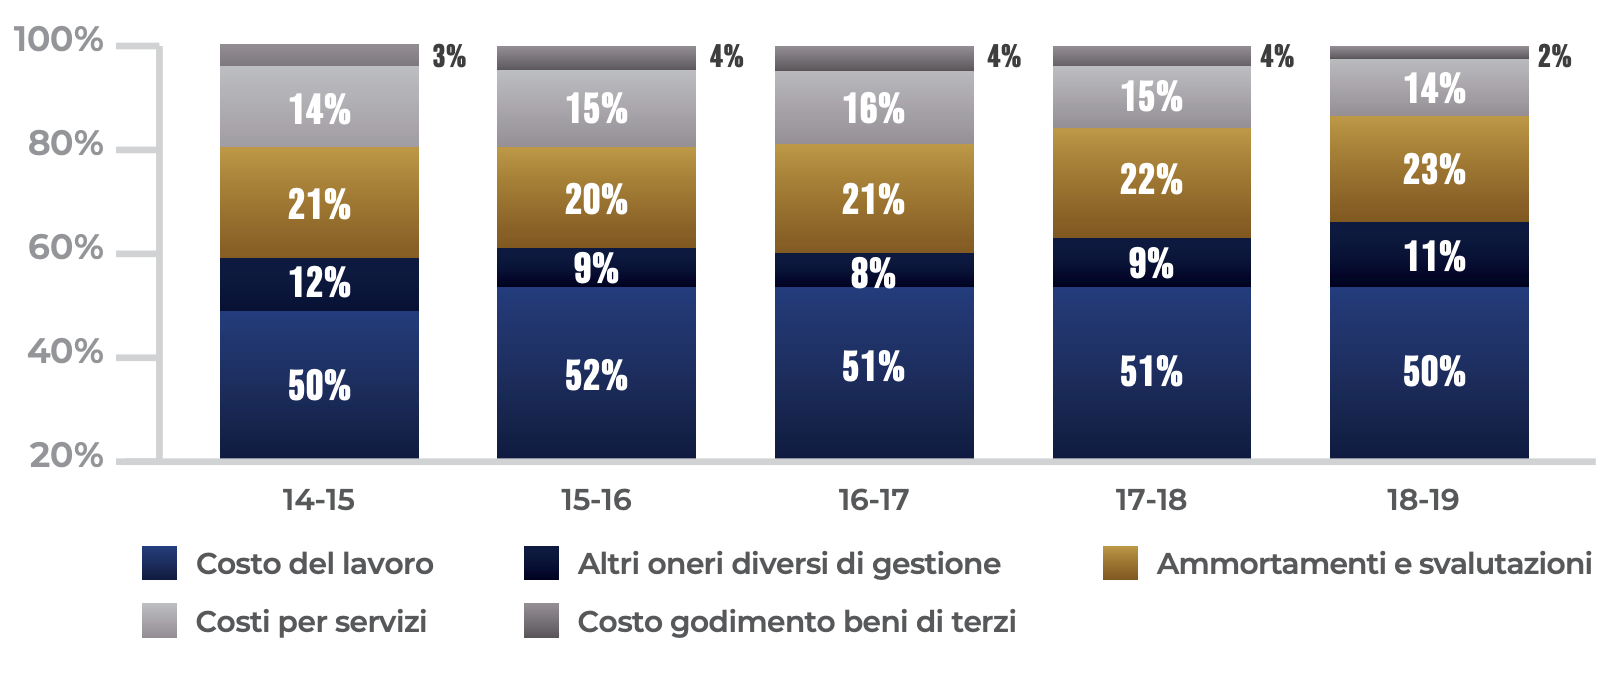
\includegraphics[width=.55\textwidth]{img/wage_serieA.png} \label{figA}} \quad
    \subfloat[][Confronto stipendi Serie A 17/18 e 18/19]
    {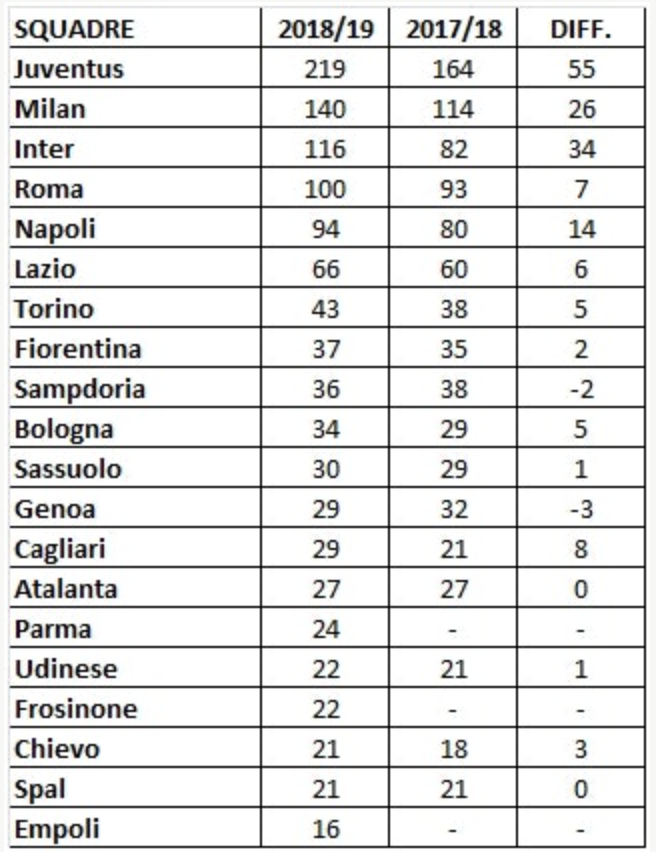
\includegraphics[width=.25\textwidth]{img/diff_wage_serieA.png} \label{figB}}
    \caption{Situazione \emph{Costo del Lavoro} all'interno del calcio italiano}
    \label{wage_serieA}  
\end{figure}\newline
Per quanto riguarda invece la \textbf{Francia}, l'organizzazione che si occupa del monitoraggio e la supervisione dei conti 
delle società calcistiche è la DNCG\footnote{Direction Nationale du Contrôle de Gestion}. Essa 
pubblica ogni stagione un report riassuntivo per quanto riguarda la Ligue 1 e la Ligue 2 (i primi due campionati) ed una
relazione relativa ad ogni singolo club dei due campionati. Tutti i dati di seguito riportati sono stati reperiti dai singoli
report annuali pubblicati\footnote{https://www.lfp.fr/dncg/rapports} \newline 
La perdita registrata nella stagione 18/19 che ammontava a 126mln€ \'e la seconda in termini di importanza a partire dal 2013/2014,
il motivo principale che spiega questa discesa cos\'i decisa \'e da attribuirsi ad un aumento delle entrate (\emph{Income})
da 304mln€ nel 17/18 a 316mln€ nel 18/19, che per\'o non riesce a contrastare l'aumento pi\'u elevato
delle spese (\emph{Expenses}) sopratutto nella sezione dedicata agli stipendi di giocatori e commissioni degli agenti 
dove troviamo un aumento rispetto all'anno precedente di 9mln€.\newline
Il secondo indicatore che viene preso in considerazione \'e chiamato \textbf{Payroll}, termine indicante la somma dei vari stipendi
dei dipendenti di un club. Nonostante un Payroll, almeno per quanto riguarda le squadre qualificate per la UCL\footnote{Uefa Champions League}, in linea con gli
altri campionati (147 mln€ nella Premier League inglese\footnote{Calcolo personale utilizzando i dati da https://www.spotrac.com/epl/payroll/}),
i risultati ottenuti nelle competizioni internazionali non sono state all'altezza: nella stagione 2018/2019 sono presenti 3 squadre 
all'interno della fase a gironi della massima competizione europea: Monaco, Paris Saint Germain e Olympique Lione. La prima si 
posizione ultima nel gruppo A, la seconda (da cui gli esperti e i sostenitori si aspettano grandi risultati, visti i milioni di euro 
spesi ogni anno) viene eliminata agli ottavi di finale e infine la terza viene anch'essa eliminata agli ottavi di finale. Questo scenario
si ripete mediamente ogni anno, in aggiunta, se si vuole trovare una squadra francese vincitrice della massima competizione europea 
dobbiamo tornare indietro alla stagione 1992/1993 con l'Olympique Marsiglia. La figura \ref{stipendi_ligue1} permette di capire, 
oltre alla disparit\'a di risorse in possesso dei club in Francia, anche il livello di spesa dei club per gli stipendi, che come \'e stato detto in precedenza non viaggia 
di pari passo ai traguardi interazionali.\newline
\begin{figure}
    \centering
    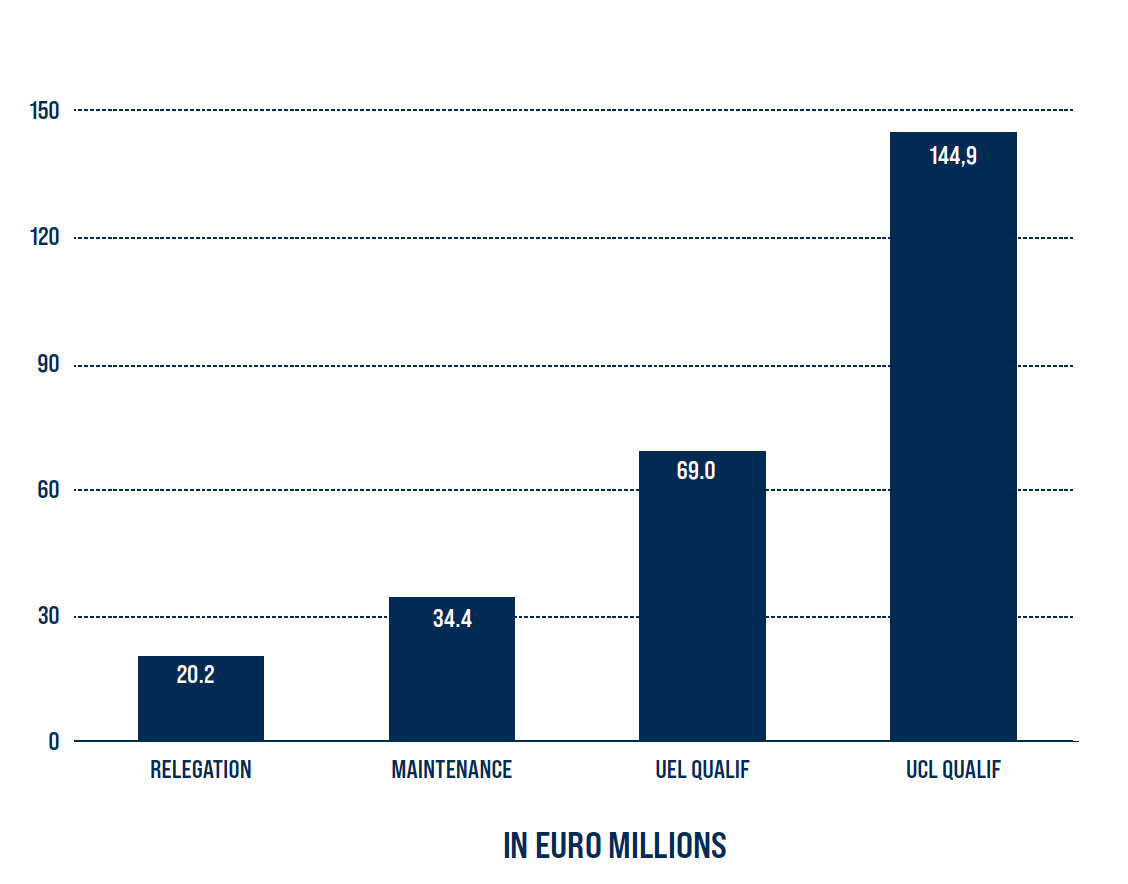
\includegraphics[scale=0.5]{img/stipendi_ligue1.png}
    \caption{Stipendi Ligue 1 a seconda del piazzamento in classifica}
    \label{stipendi_ligue1}
\end{figure}
Riprendendo l'ultimo indicatore analizzato e collegandolo al primo \'e possibile sviluppare uno scenario simile all'Italia, dove
i grandi investimenti non portano al successo assicurato e quindi ad un ritorno concreto. Queste grosse somme che escono dalle casse 
dei club che non vedono un ritorno portano un danno a tutto il campionato, all'interno del quale aumenta il gap tecnico tra le diverse squadre dello
stesso campionato mentre dall'altro, in campo internazionale, non si ottengono risultati non ricevendo quindi premi da sponsor e organizzatori.
Tutto questo circolarit\'a non fa' altro che danneggiare il sistema calcio francese facendogli perdere valore e \emph{appeal}.\newline
Il terzo Paese e di conseguenza ambiente calcistico che verr\'a analizzato \'e la \textbf{Germania}, nella quale al suo interno troviamo 
la \emph{Bundesliga} e la \emph{2.Bundesliga} che vengono a loro volta riuniti sotto la DFL\footnote{Wikipedia: Deutsche Fußball Liga}, la
federazione calcistica tedesca.\newline
Questo campionato, come pochi in Europa, possiede davvero poche criticit\'a. Iniziando con l'analisi del risultato, 
esso \'e uno degli elementi che pi\'u di tutti gli altri viene pubblicizzato 
da parte della Lega stessa all'interno del Report Annuale: 4.82 mld€ di ricavo generato dai primi due campionati nazionali in un 
solo anno, un grande traguardo raggiunto e che rimane inoltre un primato da 15 anni consecutivi
\footnote{https://www.dfl.de/en/2018-dfl-report/}.\newline
I \textbf{Ricavi} dei due massimi campionati tedeschi sono cresciuti da 2.59 mld€ nel 2016/2017 a, come detto in precedenza, 4.82 mld€ nel 2018/2019, 
registrando quindi un incremento dell'85,32\% nei 5 anni e dell'8,5\% rispetto
all'anno precedente, un risultato davvero notevole. Entrando nel dettaglio, sono aumentati i ricavi dai media grazie ai maggiori contratti nazionali 
siglati dalla stagione precedente, tuttavia, sono diminuiti anche se di poco,
i ricavi da pubblicit\'a e incontri, imputabile in modo prevalente ad un cambio della composizione del campionato stesso.
Questi ottimi risultati vengono anche supportati dal numero dei club con risultato positivo a fine esercizio: 28 su 36 (considerando 
Bundesliga e 2.Bundesliga) nel 2018/2019, mostrando come in questo Paese tutte le societ\'a, partendo dalle pi\'u virtuose,
fino ad arrivare a realt\'a pi\'u modeste hanno come primo obiettivo il creare valore.\newline
Passando alla seconda parte dell'analisi, \textbf{gli stipendi} non seguono lo stesso ragionamento fatto poco prima: la figura 
\ref{comparazione_stipendi_germania} mostra come, nonstante il valore complessivo degli stipendi dei calciatori e staff sia cresciuto in entrambi
i campionati, il totale della Bundesliga sia circa maggiore di 7 volte rispetto al campionato minore, andando quindi a dimostrare
un grande scalino di differenza tra le due leghe.
\begin{figure}
    \centering
    \subfloat[][Bundesliga]
    {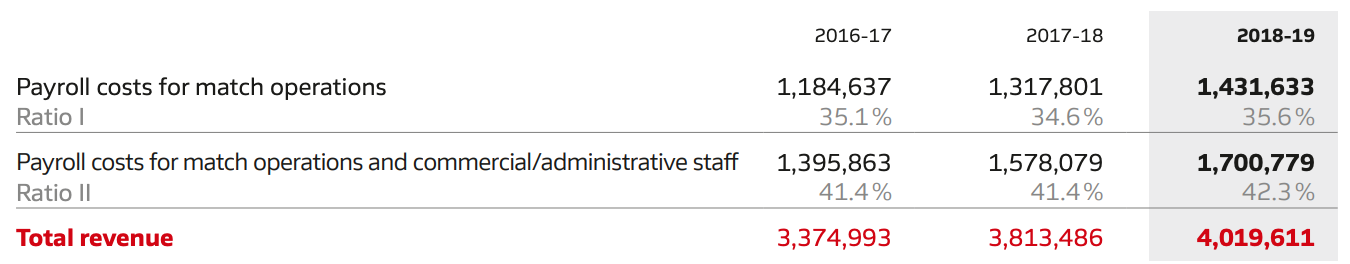
\includegraphics[width=.65\textwidth]{img/wage_germanyA.png} \label{wage_germanyA}} \quad
    \subfloat[][2.Bundesliga]
    {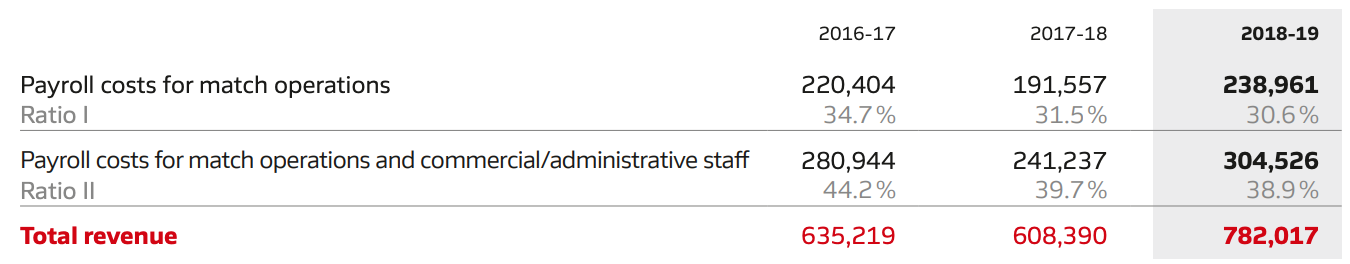
\includegraphics[width=.65\textwidth]{img/wage_germanyB.png} \label{wage_germanyB}}
    \caption{Comparazione stipendi con storico}
    \label{comparazione_stipendi_germania}  
\end{figure}
In Germania \'e radicata sicuramente una cultura legata alla precisione e al rispetto sia delle leggi che delle persone, questo si riflette 
ovviamente in tutti gli ambiti compreso quello del calcio. Come \'e possibile notare, in questo caso, i club prestano molta attenzione a non 
terminare l'anno economico con elevati debiti oppure con risultati ad un passo dal fallimento. Nonostante queste attenzioni, al contrario
di come si potrebbe pensare, arrivano anche risultati dal campo poich\'e negli ultimi anni le squadre tedesche sono sempre riuscite a ritagliarsi 
il proprio spazio nelle competizioni europee, spazio riempito con la vittoria della Champions League da parte del Bayern Monaco nel 2020. 
Rimane sempre per\'o il problema dell'inequit\'a degli stipendi. \'E possibile tuttavia anticipare gi\'a da ora, come in nessuno stato, non si possa
trovare similitudini in termini economici tra i primi due campionati.\newline
Come penultimo campionato oggetto dell'analisi troviamo la \textbf{Spagna}, formato dalla prima divisione \emph{La Liga Santander} e la seconda
\emph{La Liga Smartbank}\footnote{Tutti i dati provengono da: https://www.laliga.com/en-GB/transparency/economic-management/economic-report}.
Il Reddito Complessivo dei due campionati registra una crescita 
dalla stagione 2013/2014. Si parte con un valore combinato di 2.688,5mln€ e si arriva alla stagione 18/19 con un totale di 4.871,4mln€, 
un incremento dell'81,19\%. 
Suddividendo in modo settoriale il Total Income \'e possibile capire come in tutti i vari settori che compongono il Total Income 
si sia verificato un aumento rispetto agli anni precedenti, andando a mostrare quindi come il campionato spagnolo abbia vissuto una forte crescita negli ultimi 6 anni.
I settori sono:
\begin{enumerate}
    \item \textbf{Trasmissioni}: 1665,1 mln€ (+6,2\% rispetto all'anno precedente e +13,6\% in 5 anni). Questa crescita \'e dovuta sopratutto ad una distribuzione 
    centralizzata dei diritti grazie al RDL 5/2015 \footnote{Wikipedia: Real Decreto Ley è un atto avente forza di legge emanato dal Re}.
    \item \textbf{Attivit\'a commerciali}: 983,8 mln€ (+5,5\% rispetto all'anno precedente e +16,7\% in 5 anni). Comprende sponsorizzazioni,
    pubblicit\'a e merchandising.
    \item \textbf{Partite}: 948,6 mln€ (+24,4\% rispetto all'anno precedente e +9,3\% in 5 anni). Comprende le competizioni, biglietti 
    e altre entrate distribuite dalla UEFA.
\end{enumerate}
Il risultato finale del Reddito \'e stato, inoltre, favorito in modo importante dalla crescita di altri 2 fattori che caratterizzano l'attivit\'a tipica del
campionato:
\begin{enumerate}
    \item \textbf{Trasferimenti}: 1006,2 mln€ (+7,2\% rispetto all'anno precedente e +18,1\% in 5 anni).
    \item \textbf{Altre Entrate}: : 267,7 mln€ (+15,7\% rispetto all'anno precedente e -2,8\% in 5 anni). Unico valore che vede una diminuzione
    nel medio periodo ma dovuta al fatto che questa voce, comprendendo accordi di natura finanziaria, assume valori molto diversi nel corso degli anni.
\end{enumerate}
Spostandosi al secondo tema, anche in questo caso come per l'Italia, non viene elaborata un'analisi dettagliata degli stipendi. Nel documento
viene indicato solamente il costo degli stipendi nel corso degli anni e il suo rapporto in percentuale con il Reddito Complessivo e il Fatturato Netto
(figura \ref{wage_spain}).
\begin{figure}
    \centering
    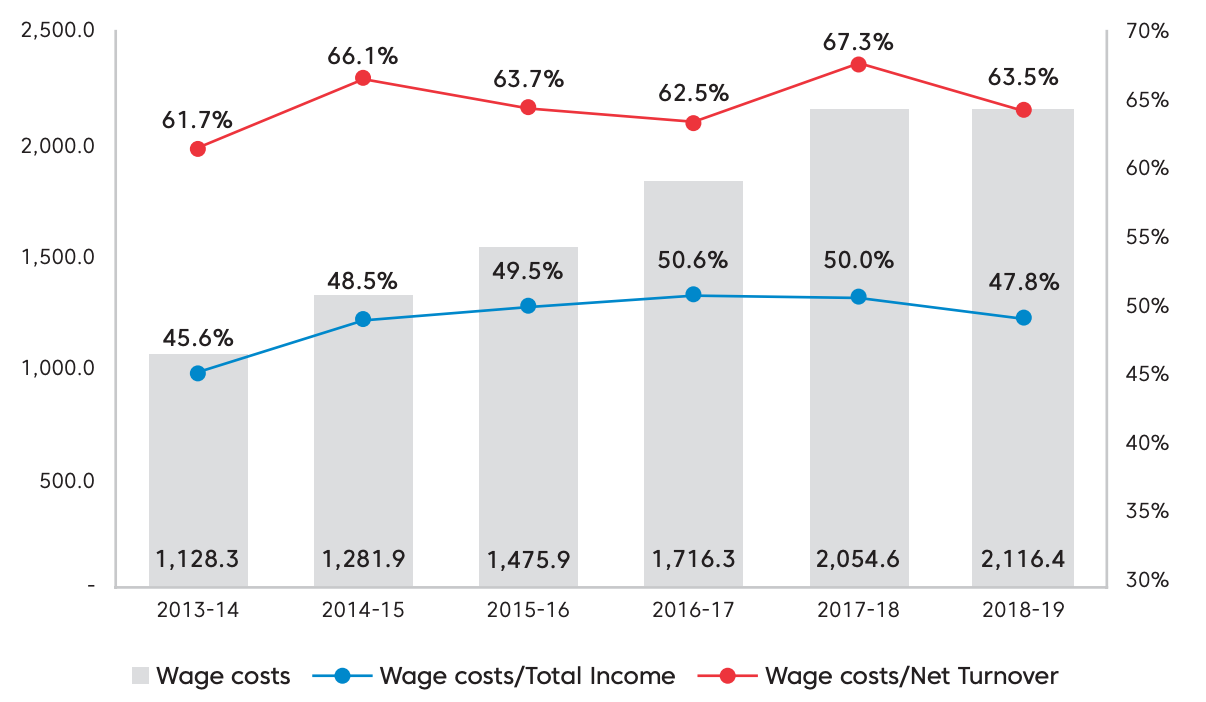
\includegraphics[scale=.5]{img/wage_spain.png}
    \caption{Stipendi La Liga}
    \label{wage_spain}
\end{figure}
La figura mostra come nonostante l'aumento del costo degli stipendi sul totale dei costi, il rapporto con il fatturato vada di anno in anno
a decrescere, mostrando ancora una volta come il campionato spagnolo sia in crescita economica. Un risultato nuovamente positivo \'e stato
sicuramente influenzato dal \emph{\textbf{Salary Cap}} introdotta nel 2013 da parte del CdS\footnote{Wikipedia: Consejo Superior de Deportes cio\'e il massimo organo sportivo a livello nazionale}.
Questa nuova riforma ha il campito di porre dei limiti alle spese dei club riguardo gli stipendi e in generale tutti i costi connessi ai calciatori,
per evitare problematiche presenti ad esempio in Francia dove club con forti disponibilit\'a economiche gareggiano incontrastati nel Paese.\newline
Dovendo fornire un commento/conclusione all'analisi appena svolta \'e possibile affermare come La Liga sia innegabilmente in crescita da 6 
anni a questa parte, essendo il secondo campionato pi\'u visto al mondo con 2.663 mln di spettatori, dietro solo la Premier League a quota 
3.200 mln\footnote{Premier League: https://www.premierleague.com/news/1280062}.\newline
Come ultimo elemento compreso in questa prima analisi suddivisa per Paesi troviamo l'\textbf{Inghilterra}. In questo Paese il calcio 
\'e una vera e propria colonna portante, capace di generare ricavi per 5.440mln£\footnote{https://www2.deloitte.com/global/en/pages/about-deloitte/articles/annual-review-of-football-finance.html}
nella stagione 2017/2018. Il punto di forza \'e sicuramente legato alla vastissima diffusione dei diritti tv che compongono il fattore ricavi
del 59\% ma \'e anche, sopratutto, una questione di lingua dato che l'inglese \'e la lingua pi\'u diffusa in tutto il mondo.\newline
Iniziando a presentare i dati riguardanti l'analisi, la societ\'a Deloitte tramite l'\emph{Annual Review of Football Finance} mostra
l'andamento dei 5 maggiori campionati europei e si sofferma inoltre su quello inglese. Questo report mostra come in solo 3 anni i \textbf{ricavi} 
dei club di \emph{Premier League}, il primo campionato inglese, siano aumentati del 41,71\% passando da 3.639mln£ a 5.157mln£ valori a cui solo
la Bundesliga riesce quantomeno ad avvicinarcisi. Il punto di forza, come gi\'a affermato prima, \'e sicuramente i ricavi generati dai diritti
tv che compongono ogni anni pi\'u della met\'a dei ricavi totali; anche la parte denominata \emph{Commercial} non \'e da meno, con valori
che si aggirano sempre intorno ai 1.500mln£. Il vero problema per\'o si presenta se si va a confrontare i ricavi dei cosiddetti \emph{Big Six}, 
i 6 club che hanno fatto la storia del campionato: Arsenal, Manchester City, Manchester United, Tottenham, Chelsea e Liverpool con i ricavi
generati dalle altre societ\'a.
\begin{figure}
    \centering
    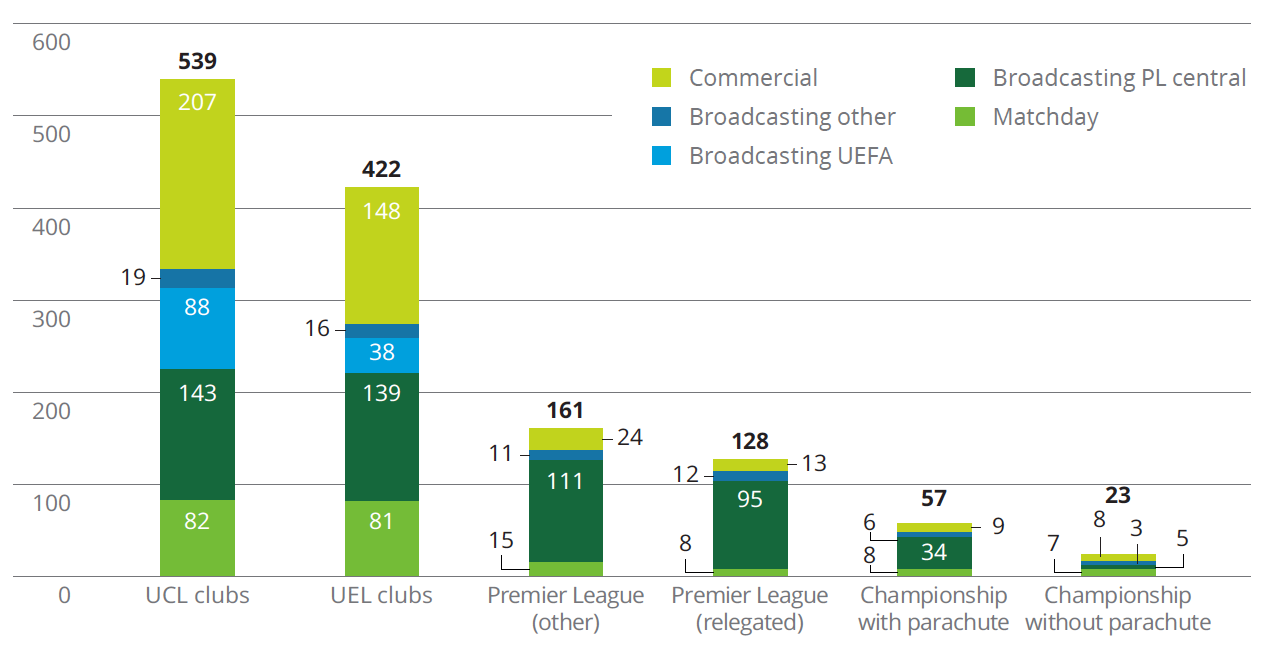
\includegraphics[scale=0.5]{img/ricavi_premier.png}
    \caption{Confronto ricavi dei club di Premier League divisi per gruppi}
    \label{ricavi_premier}
\end{figure} 
La figuta \ref{ricavi_premier} permette di visualizzare immediatamente questa differenza. L'ultima classificata tra i \emph{Big Six},
l'Arsenal ha generato ricavi 393mln£ mentre il West Ham, classificatosi settimo e quindi una posizione immediatamente sotto l'Arsenal, ha 
prodotto per 193mln£, una differenza di ricavi di 200mln£ con una sola posizione in classifica di distacco. Nel grafico sono inoltre riportati
i club retrocessi "con paracadute", un sistema che tramite i diritti di trasmissione aiuta economicamente i club nelle posizioni
pi\'u basse della classifica.\newline
Sempre all'intrerno dell'analisi prodotta da Deloitte \'e contenuto un approfondimento sugli \textbf{stipendi}. Anche in questo caso, se a
primo impatto i dati non sembrano preoccupare, se si analizzano a fondo si pu\'o notare come gi\'a dalla stagione 2018/2019 ci fossero segni
di preoccupazione. Il peso degli stipendi per i club della Premier League in quella stagione ammontava a 3.155mln£, il 61\% dei ricavi contro il 
59\% dell'anno precedente. Questo aumento ha fatto si che si presentassero alla fine dell'esercizio ben 6 club con una perdita operativa, il 
peggior risultato dal 2012/2013.\newline
\section{Analisi per Club}
La seconda parte di questa trattazione andr\'a a prendere in esame i club pi\'u importanti oppure quelli che saranno pi\'u utili al fine 
delle successive analisi dei diversi Paesi elencati nel sottocapitolo precedente. Per quanto riguarda l'Italia verr\'a analizzata la \textbf{Juventus},
per la Francia il \textbf{Paris Saint Germain}, per la Germania il \textbf{Borussia Dortmund}, per la Spagna il \textbf{Barcellona} e infine per l'Inghilterra il 
\textbf{Manchester City}.\newline
L'analisi verr\'a svolta considerando 4 macro-categorie:
\begin{enumerate}
    \item Analisi dei Ricavi: similmente a come fatto prima ma in modo pi\'u specifico, in questa parte verr\'a fatta un'analisi relativa
        ai diversi tipi di ricavo e la loro incidenza rispetto ai ricavi totali; 
    \item Analisi della Liquidit\'a: in questa sezione verranno analizzate le voci di bilancio relative agli impegni delle societ\'a
        nel breve/medio periodo;
    \item Analisi della Solidit\'a: qu\'i invece verranno prese in analisi le capacit\'a dei club di far fronte ad impegni su un periodo di
        tempo pi\'u lungo, evidenziando o meno il peso dei mezzi propri e la dipendenza dai finanziatori terzi;
    \item Analisi della Redditivit\'a: nella penultima categoria di analisi viene "tagliato" in modo orizzontale il bilancio, andando quindi
        a considerare sia voci di Stato Patrimoniale sia voci di Conto Economico per capire gli investimenti effettuati e i risultati ottenuti;
\end{enumerate} 
\subsection{Juventus}
Il primo club ad essere analizzato \'e appunto la Juventus, uno dei club pi\'u famosi e vincenti in Italia e tredicesima per numero di tifosi 
in tutto il mondo. Il potere \'e sempre stato in mano alla famiglia Agnelli, che a partire dal 1923 ha guidato il club torinese ad un lungo
\emph{palmares} di successi\footnote{https://it.wikipedia.org/wiki/Storia\_della\_Juventus\_Football\_Club}. Alla stagione 2018/2019 vantava: 34 Scudetti di cui dal 2012 sette conquistati consecutivamente, 13
Coppe Italia, 7 Supercoppe Italiane, 2 Champions League e 2 Coppe Intercontinentali.\newline
\begin{enumerate}
    \item Analisi dei Ricavi:\newline
        Per questa primo punto \'e necessario prendere in considerazione il prospetto di Conto Economico al 30 Giugno 2019.
        Verrano messi in relazione alcune voce della sezione ricavi del CE con il totale dei ricavi generati sottraendo per\'o la voce
        "Altri Ricavi" in modo da prendere in considerazione solo le voci pi\'u rilevanti.
        \begin{figure}
            \centering
            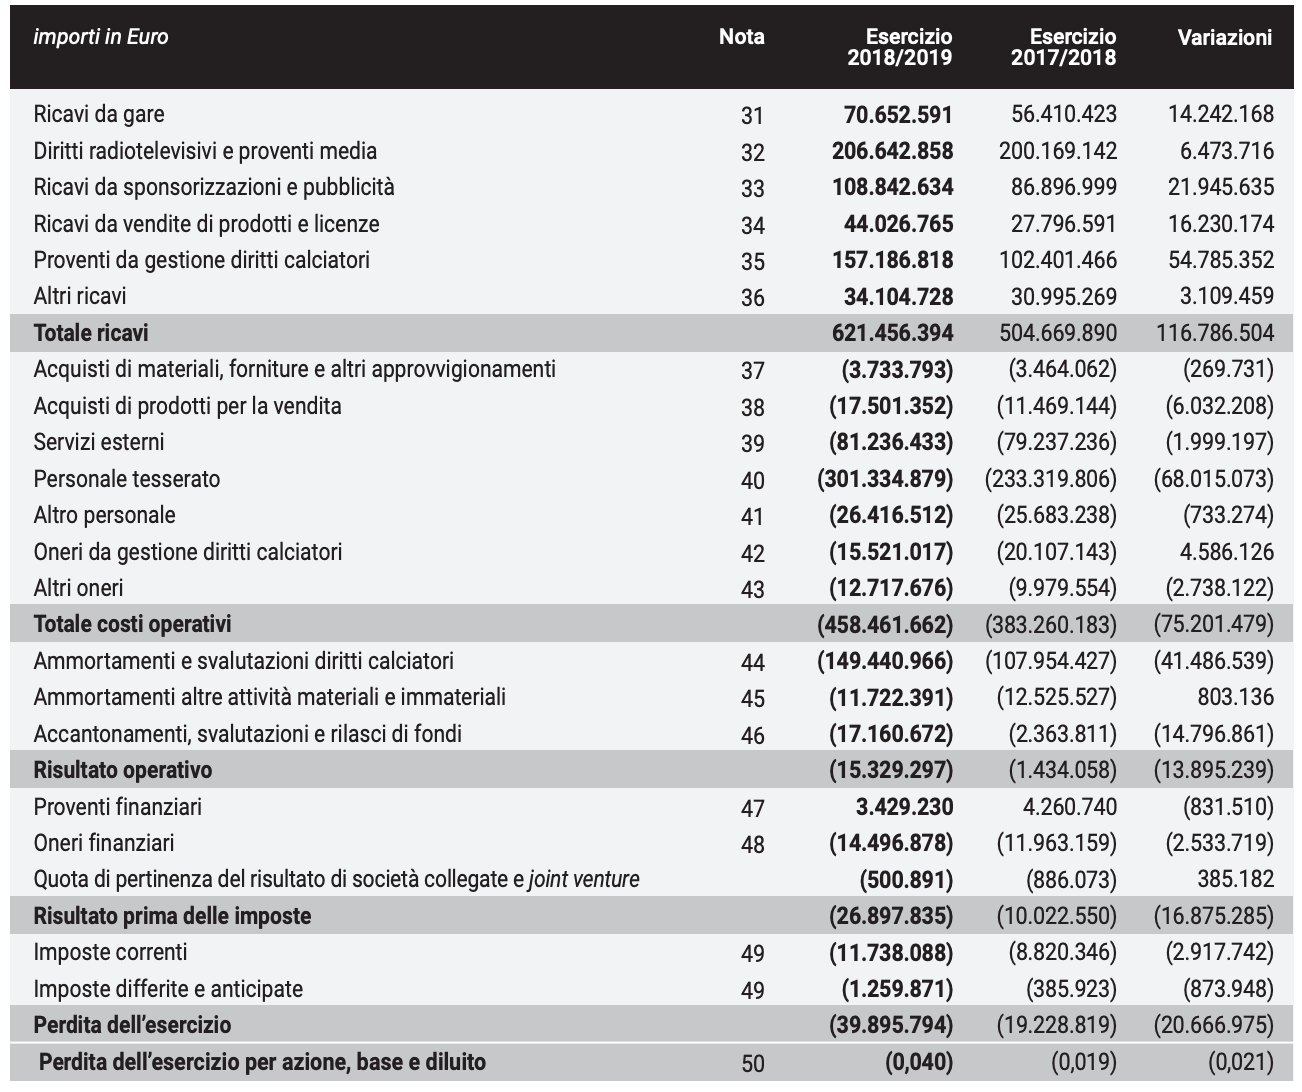
\includegraphics[scale=.4]{img/CE_juve.png}
            \caption{Conto Economico Juventus al 30 Giugno 2019}
            \label{ce_juve}
        \end{figure}\newline
        \begin{equation}
            \frac{\text{Ricavi da gare}}{\text{Totale Ricavi}} = \frac{70.652.591}{587.351.666} = \mathbf{12,02\%}
            \label{eqn: gare_juve}
        \end{equation}
        \begin{equation}
            \frac{\text{Diritti TV}}{\text{Totale Ricavi}} = \frac{206.642.858}{587.351.666} = \mathbf{35,18\%}
            \label{eqn: tv_juve}
        \end{equation}
        \begin{equation}
            \frac{\text{Ricavi commerciali}}{\text{Totale Ricavi}} = \frac{152.869.399}{587.351.666} = \mathbf{26,02\%}
            \label{eqn: commerc_juve}
        \end{equation}
        Per quanto la Juventus sia tra le poche societ\'a nel panorama italiano ad avere uno stadio di propriet\'a, 
        insieme a Udinese e Sassuolo, il profilo dei suoi ricavi non \'e minimamente paragonabile alle concorrenti Europee.
        Come si vedrà pi\'u avanti con l’analisi dei bilanci di squadre come Barcellona e Manchester City, sopratutto la voce dei Ricavi
        da Stadio e Ricavi Commerciali non \'e minimamente confrontabile. Un secondo problema che deve far allarmare la societ\'a Piemontese
        \'e il fatto che i ricavi da gare siano molto bassi a causa di una inspiegabile bassa affluenza di tifosi alla stadio. Basti pensare 
        che l'Allianz Stadium ha una media spettatori simile a quella dell'Artemio Franchi di Firenze, palcoscenico piuttosto differente da 
        quello di Torino\footnote{TransferMarket: https://www.transfermarkt.it/ac-florenz/besucherzahlenentwicklung/verein/430}.
    \item Analisi della liquidit\'a:\newline
        Per questo punto andranno invece a considerarsi le voci presenti nello Stato Patrimoniale del Bilancio d'Esercizio.
        \begin{figure}
            \centering
            \subfloat[][Stato Patrimoniale attivo al 30 Giugno 2019]
            {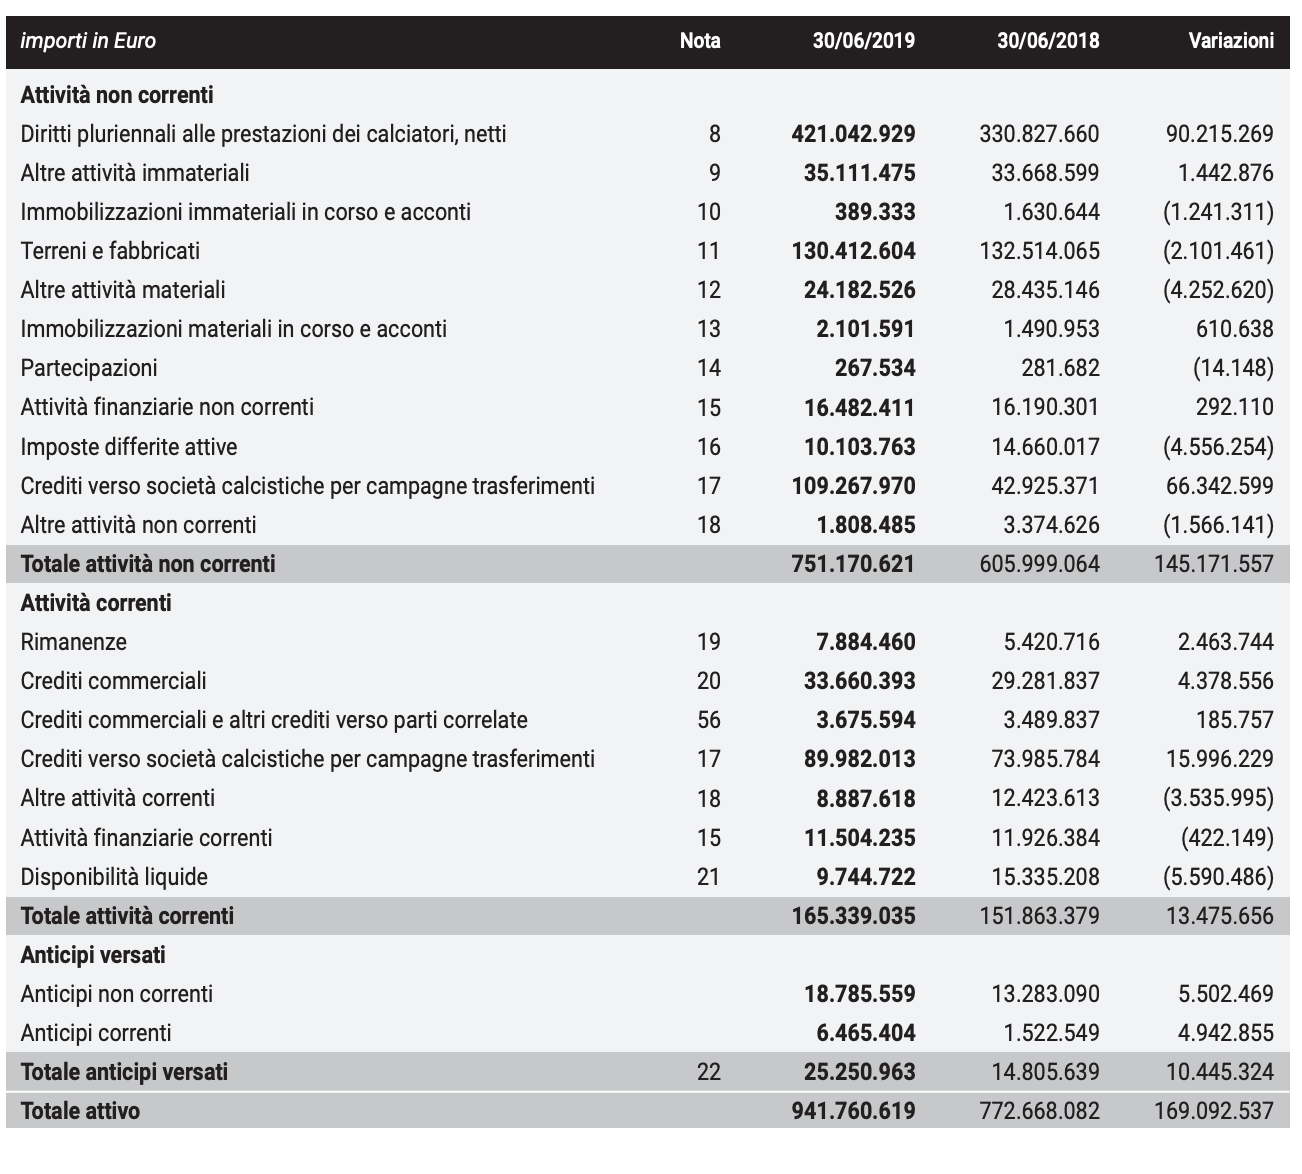
\includegraphics[width=.45\textwidth]{img/SP_attivo_juve.png} \label{sp_attivo_juve}} \quad
            \subfloat[][Stato Patrimoniale passivo al 30 Giugno 2019]
            {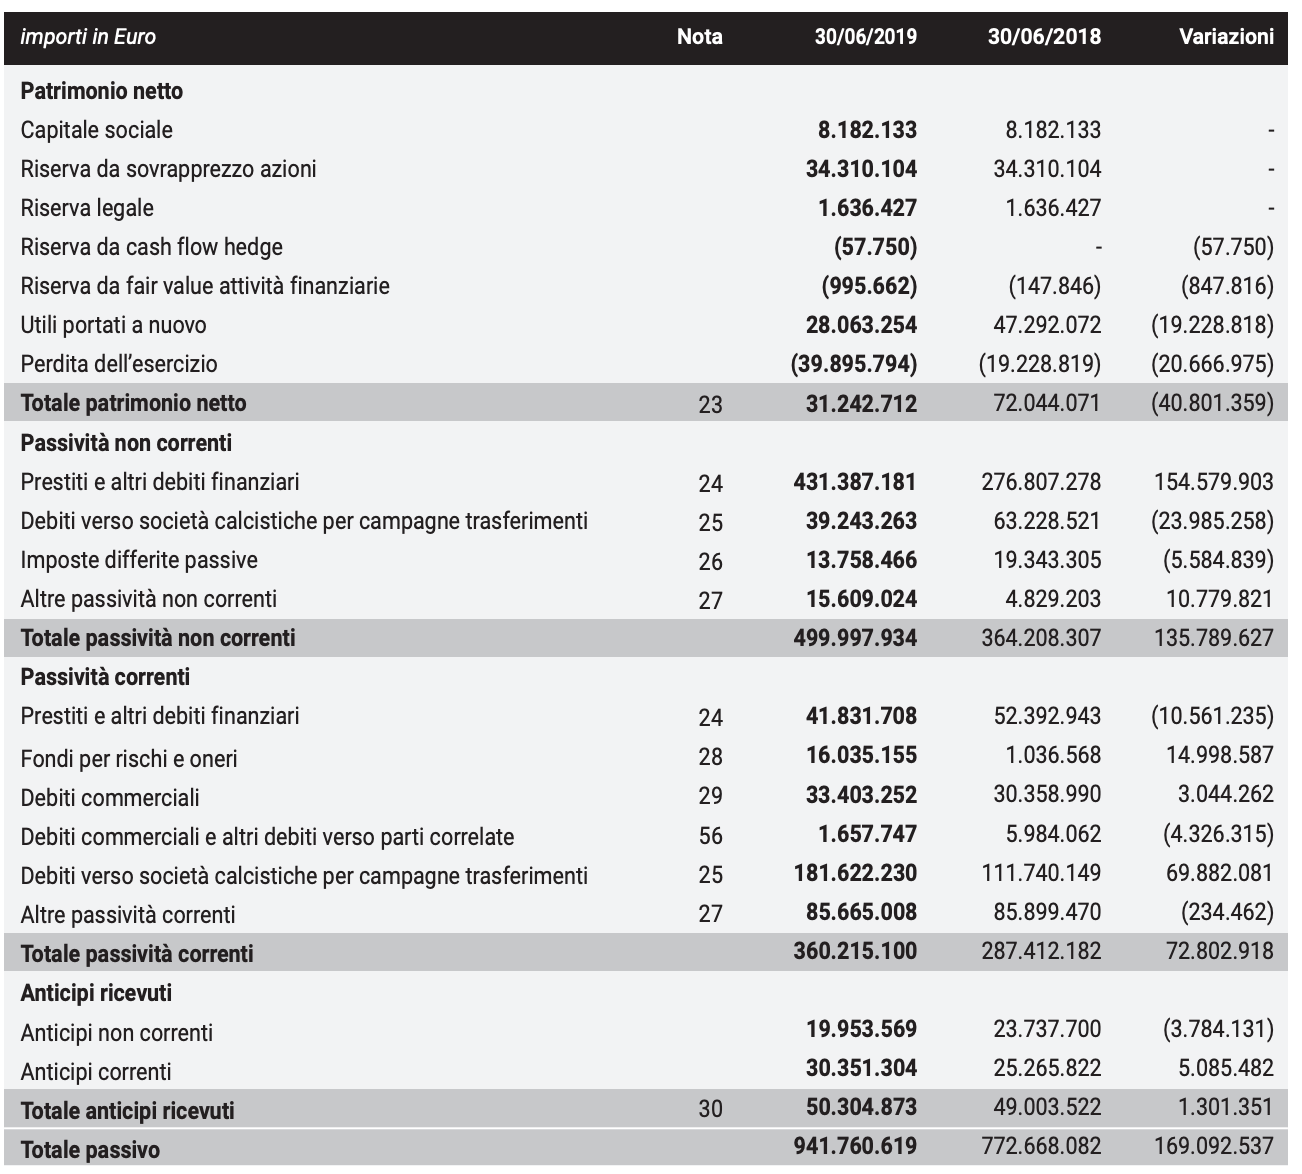
\includegraphics[width=.45\textwidth]{img/SP_passivo_juve.png} \label{sp_passivo_juve}}
            \caption{Stato Patrimoniale Juventus al 30 Giungno 2019}
            \label{sp_juve}  
        \end{figure}
        \begin{equation}
                \text{Margine di Tesoreria} = 157.454.575-390.566.404 = \mathbf{-233.111.829\mbox{\euro}}
            \label{eqn: marg_teso_juve}
        \end{equation}
        \begin{equation}
                \text{Indice di liquidit\'a primaria} = \frac{157.454.575}{390.566.404} = \mathbf{40,31\%}
            \label{eqn: ind_liq_juve}
        \end{equation}
        Per quanto riguarda l'analisi degli indici di Stato Patrimoniale che identificano quanto una societ\'a \'e in grado di far 
        fronte, con mezzi correnti e non correnti, alle passivit\'a a breve termine la situazione della Juventus non \'e del tutto positiva.
        Per essere considerato efficace il Margine di Tesoreria e il relativo Indice di Liquidit\'a primaria devono essere entrambi positivi
        e maggiori di uno\footnote{Valter Cantino, Paola De Bernardi, Alain Devalle (2018) Sistemi di rilevazione e misurazione delle performance aziendali Torino: G. Giappichelli};
        in entrambi i casi questi requisiti non vengono soddisfatti. I dati peggiorano anche rispetto all'anno precedente
        questo a causa dell'acquisto del calciatore Cristiano Ronaldo, il quale in Bilancio ha il suo peso con un 
        prezzo di acquisto di 115mln€ e uno stipendio lordo di 57mln€. Questo problema per\'o \'e risaputo: tutti i club del mondo si indebitano,
        sopratutto nei confronti dei calciatori che con il passare degli anni avanzano richieste sempre maggiori e, per far fronte a queste 
        richieste i club creano altro debito, andando a creare un vero e proprio circolo vizioso.
    \item Analisi della solidit\'a:\newline
        \begin{equation}
            \text{Grado di Indpendenza Finanziaria} = \frac{31.242.712}{941.760.619} = \mathbf{3,31\%}
        \label{eqn: indeb_juve}
        \end{equation}
        \begin{equation}
            \text{Margine di Struttura} = 31.242.712-613.240.458 = \mathbf{-581.997.746\mbox{\euro}}
            \label{eqn: marg_strutt_juve}
        \end{equation}
        In questa sezione la Juventus presenta due situazioni nuovamente negative: a causa del risultato in rosso dell'anno
        precedente il Patrimonio Netto \'e diminuito e di conseguenza il grado di indipendenza finanziaria si attesta al 3,31\%,
        un valore che mostra la dipendenza della societ\'a da mezzi esterni; il Margine di Struttura
        visualizza invece la capacit\'a dei mezzi propri di coprire le immobilizzazioni e capire se serve ricorrere a mezzi terzi. Anche in questo 
        caso un valore negativo \'e preoccupante perch\'e sta a significare che per quasi 600mln€ serviranno mezzi terzi.\newpage
    \item Analisi della Redditivit\'a:\newline
        \begin{equation}
            \text{ROI} = \frac{-15.329.297}{941.760.619} = \mathbf{-1,6\%}
        \label{eqn: roi_juve}
        \end{equation}
        \begin{equation}
            \text{ROE} = \frac{-39.895.794}{31.242.712} = \mathbf{-127,69\%}
        \label{eqn: roe_juve}
        \end{equation}
        Questo ultimo punto dell'analisi evidenzia in modo immediato come la societ\'a stia rischiando molto in campo economico: troviamo in 
        primo luogo un peggioramento significativo del Reddito Operativo che passa da -1.434.058€ nel 2017 a -15.239.297€ nel 2018 (una variazione del 962\%);
        anche la perdita d'esercizio ha un andmento simile con uno scostamento di 20mln€ rispetto all'anno precedente. Questo peggioramento
        cos\'i importante dei valori \'e dovuto sopratutto all'aumento del personale tesserato e alla voce "Ammortamenti e svalutazione diritti calciatori",
        sempre legata all'acquisto di Cristiano Ronaldo.
\end{enumerate}
\subsection{Paris Saint Germain}
Spostandosi in Francia troviamo il Paris Saint Germain, squadra famosa in tutto il mondo grazie alla potenza economica dello sceicco Nasser Al-Khelaïfi 
che, nel 2011\footnote{Wikipedia: https://it.wikipedia.org/wiki/Nasser\_Al-Khela\%C3\%AFfi}, acquista la maggioranza delle quote della societ\'a e da il via 
ad un periodo di spese folli per creare un vero e proprio impero.
Queste cifre spese non sono per\'o servite ad ottenere risultati significativi, l'unico traguardo degno di nota della squadra dal 2011 ad oggi
\'e stata la finale di Champions League nel 2020, persa con il Bayern Monaco.\newpage
\begin{enumerate}
    \item Analisi dei Ricavi:\newline
        \begin{figure}
            \centering
            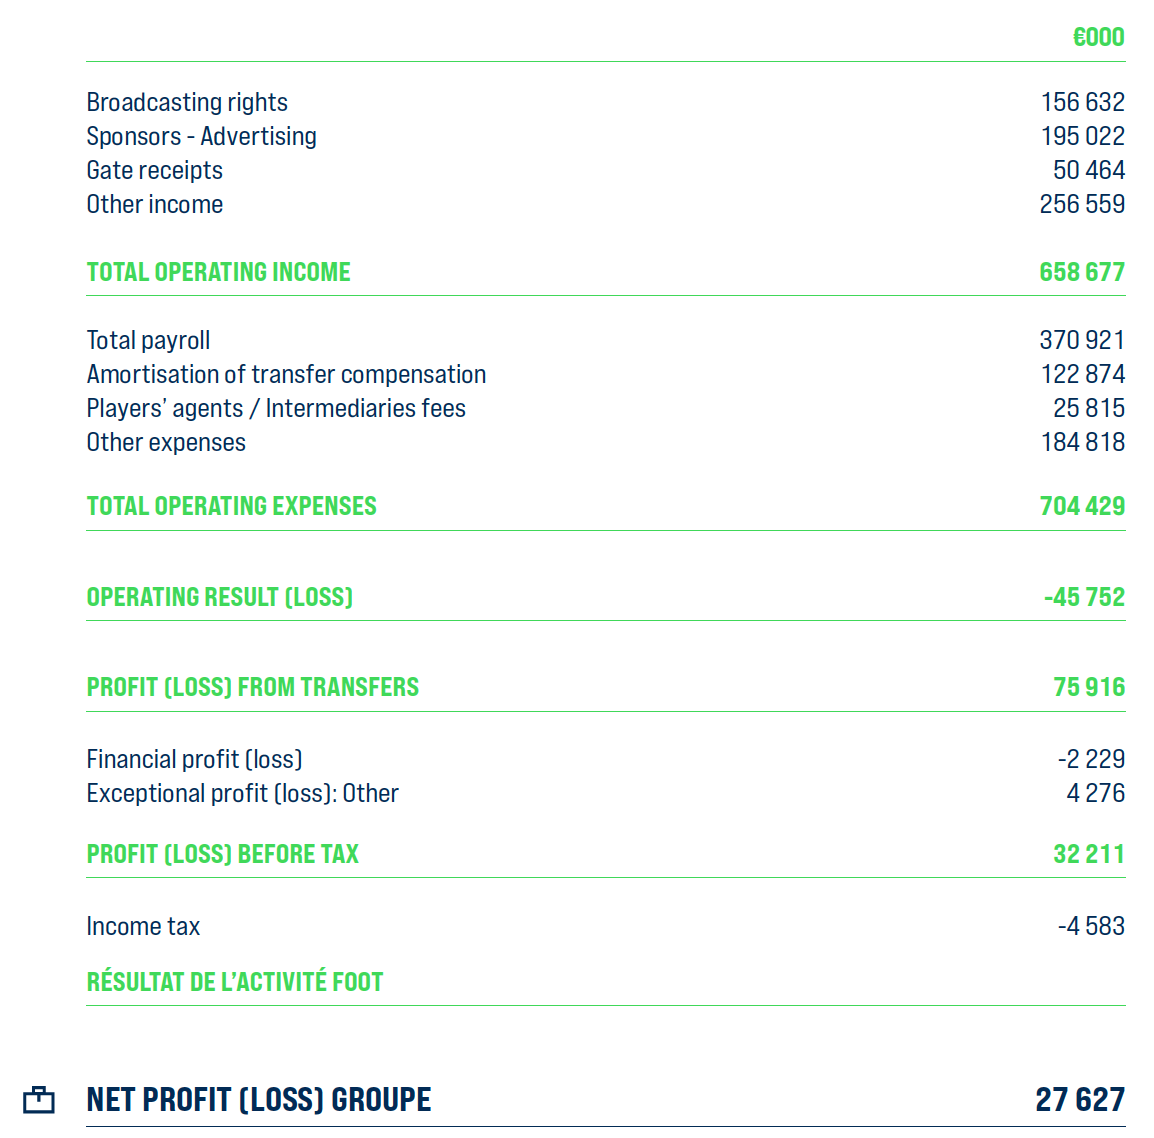
\includegraphics[scale=.4]{img/CE_psg.png}
            \caption{Conto Economico Paris Saint Germain al 30 Giugno 2019}
            \label{ce_psg}
        \end{figure}\newline
        \begin{equation}
            \frac{\text{Ricavi da gare}}{\text{Totale Ricavi}} = \frac{50.464.000}{658.677.000} = \mathbf{7,68\%}
            \label{eqn: gare_psg}
        \end{equation}
        \begin{equation}
            \frac{\text{Diritti TV}}{\text{Totale Ricavi}} = \frac{156.632.000}{658.677.000} = \mathbf{23,77\%}
            \label{eqn: tv_psg}
        \end{equation}
        \begin{equation}
            \frac{\text{Ricavi commerciali}}{\text{Totale Ricavi}} = \frac{195.022.000}{658.677.000} = \mathbf{29,60\%}
            \label{eqn: commerc_psg}
        \end{equation}
        In questo scenario troviamo una situazione abbastanza differente. Sebbene il Paris Saint Germain sia molto seguita in Europa e nel
        mondo i ricavi da gare e diritti Tv sono inferiori (rapportati al Totale Incassi) rispetto a quelli della Juventus\footnote{https://www.lfp.fr/dncg/rapports}: questo perch\'e
        in Francia non troviamo una cos\'i radicata cultura calcistica, sopratutto per quanto riguarda i singoli club e, mancando di \emph{appeal}
        internazionale, il campionato francese non pu\'o contare molto sulla vendita della trasmissione delle partite. I Ricavi Commerciali invece
        sono leggermente superiori per il motivo appunto che data la grande importanza a livello mondiale del club, esso vende maggiormente in tutto il mondo.
    \item Analisi della liquidit\'a:\newline
        \begin{figure}
            \centering
            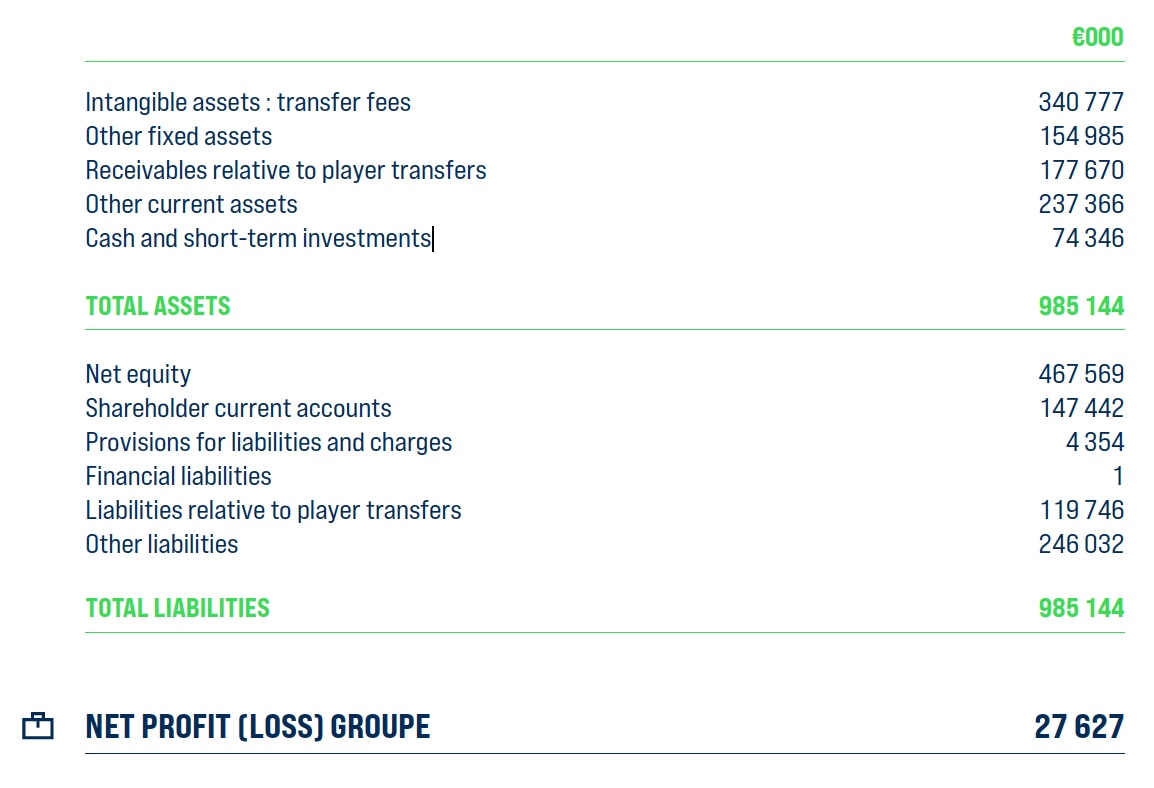
\includegraphics[scale=.5]{img/SP_psg.png}
            \caption{Stato Patrimoniale Paris Saint Germain al 30 Giungno 2019}
            \label{sp_psg}  
        \end{figure}
        \begin{equation}
                \text{Margine di Tesoreria} = 74.346.000-246.032.000 = \mathbf{-171.786.000\mbox{\euro}}
            \label{eqn: marg_teso_psg}
        \end{equation}
        \begin{equation}
                \text{Indice di liquidit\'a primaria} = \frac{74.346.000}{246.032.000} = \mathbf{30,21\%}
            \label{eqn: ind_liq_psg}
        \end{equation}
       Anche in questo caso non si presenta una situazione positiva: l'equazione \ref{eqn: marg_teso_psg} mostra come anche in questo caso il 
       risultato sia negativo, anche se in valore minore. Questo probabilmente perch\'e il PSG possedendo una quantit\'a elevatissima di risorse
       liquide e immediate, riesce comunque a tenere sotto controllo le passivit\'a a breve termine.
    \item Analisi della solidit\'a:\newline
        \begin{equation}
            \text{Grado di Indipendenza finanziaria} = \frac{467.569.000}{985.144.000} = \mathbf{47,46\%}
        \label{eqn: indeb_psg}
        \end{equation}
        \begin{equation}
            \text{Margine di Struttura} = 467.569.000-495.762.000 = \mathbf{-28.193.000\mbox{\euro}}
            \label{eqn: marg_strutt_psg}
        \end{equation}
        Contrariamente a quanto si \'e visto per la Juventus, la squadra di Parigi \'e maggiormente in grado di affrontare
        debiti e passivit\'a finanziarie tramite il capitale proprio, questo accade sicuramente grazie alla forte capitalizzazione
        che apporta il presidente. Tramite il margine di struttura, invece, possiamo capire come anche in questo caso, con solo mezzi propri non si riesca a coprire il valore
        delle immobilizzazioni anche se, 28mln€ di differenza non sono cos\'i elevati considerando i numeri di oggi.
    \item Analisi della Redditivit\'a:\newline
        \begin{equation}
            \text{ROI} = \frac{-45.752.000}{985.144.000} = \mathbf{-4,6\%}
        \label{eqn: roi_psg}
        \end{equation}
        \begin{equation}
            \text{ROE} = \frac{27.627.000}{467.569.000} = \mathbf{5,90\%}
        \label{eqn: roe_psg}
        \end{equation}
        Questo ultimo punto dell'analisi mette in mostra due risultati molto differenti: da una parte troviamo un ROI negativo dovuto ad
        un risultato netto negativo a causa della grande spesa per gli stipendi (370.921.000€) ed un Capitale Investito anch'esso molto elevato;
        dall'altro lato invece il ROE assume un valore positivo, anche se non ancora considerabile buono, grazie al profitto generato dalla 
        vendita dei giocatori e dalla non elevata tassazione applicata in Francia
\end{enumerate}
\subsection{Borussia Dortmund}
Continuando la disamina dei vari club Europei, ora \'e il momento del Borussia Dortmund. Il club tedesco anche se spesso oscurato dai continui
successi del Bayern Monaco è comunque riuscito a ritagliarsi il suo spazio in patria e in Europa, conquistando: 8 campionati tedeschi, 5 supercoppe di Germania, 4 coppe nazionali, 1 Champions League e 1 Coppa
intercontinentale\footnote{https://it.wikipedia.org/wiki/Ballspielverein\_Borussia\_09\_Dortmund}. 
\begin{enumerate}
    \item Analisi dei Ricavi:\newline
        \begin{figure}
            \centering
            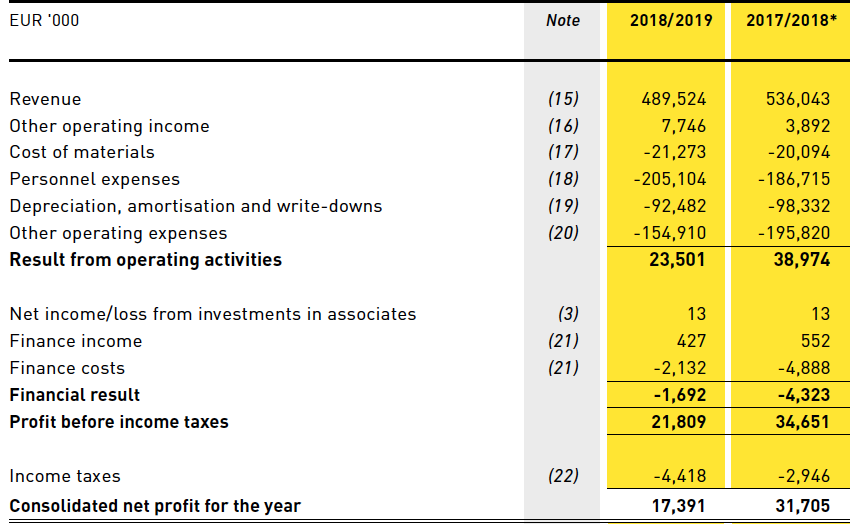
\includegraphics[scale=.4]{img/CE_dor.png}
            \caption{Conto Economico Borussia Dortmund al 30 Giugno 2019}
            \label{ce_dor}
        \end{figure}\newline
        \begin{equation}
            \frac{\text{Ricavi da gare}}{\text{Totale Ricavi}} = \frac{44.659.000}{498.777.000} = \mathbf{8,95\%}
            \label{eqn: gare_dor}
        \end{equation}
        \begin{equation}
            \frac{\text{Diritti TV}}{\text{Totale Ricavi}} = \frac{167.349.000}{498.777.000} = \mathbf{33,55\%}
            \label{eqn: tv_dor}
        \end{equation}
        \begin{equation}
            \frac{\text{Ricavi commerciali}}{\text{Totale Ricavi}} = \frac{130.002.000}{498.777.000} = \mathbf{26,06\%}
            \label{eqn: commerc_dor}
        \end{equation}
        In Germania la situazione \'e abbastanza analoga come per l'Italia: i ricavi da gare sono pi\'u bassi ma salgono rispetto all'anno precedente,
        i ricavi da diritti tv rimangono sulla stessa linea ma scendono di qualche punto percentuale anche i ricavi commerciali, probabilmente
        per il fatto che il Borussia non \'e cos\'i largamente conosciuto nel mondo come pu\'o esserlo la Juventus.
    \item Analisi della liquidit\'a:\newline
        \begin{figure}
            \centering
            \subfloat[][Stato Patrimoniale attivo al 30 Giugno 2019]
            {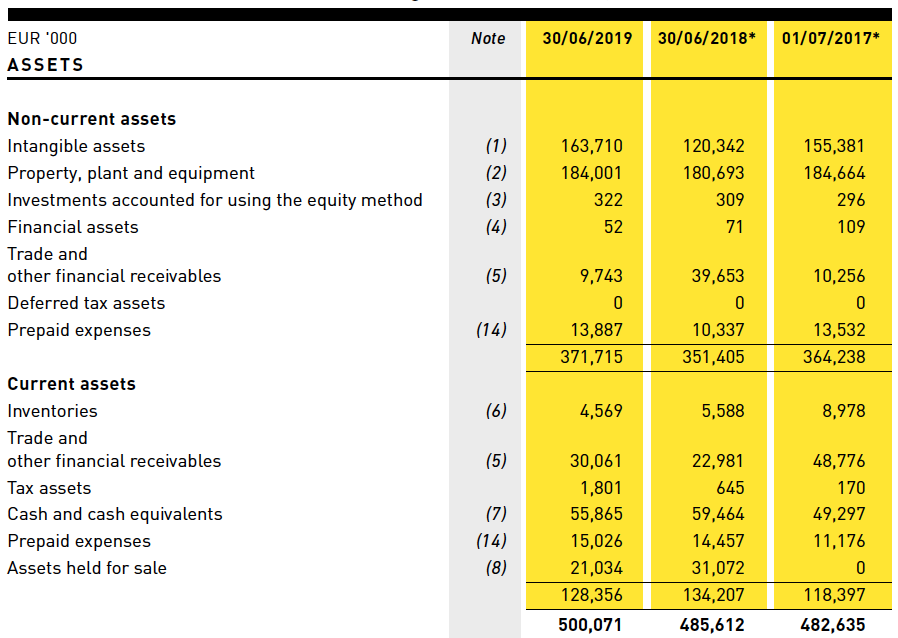
\includegraphics[width=.45\textwidth]{img/SP_attivo_dor.png} \label{sp_attivo_dor}} \quad
            \subfloat[][Stato Patrimoniale passivo al 30 Giugno 2019]
            {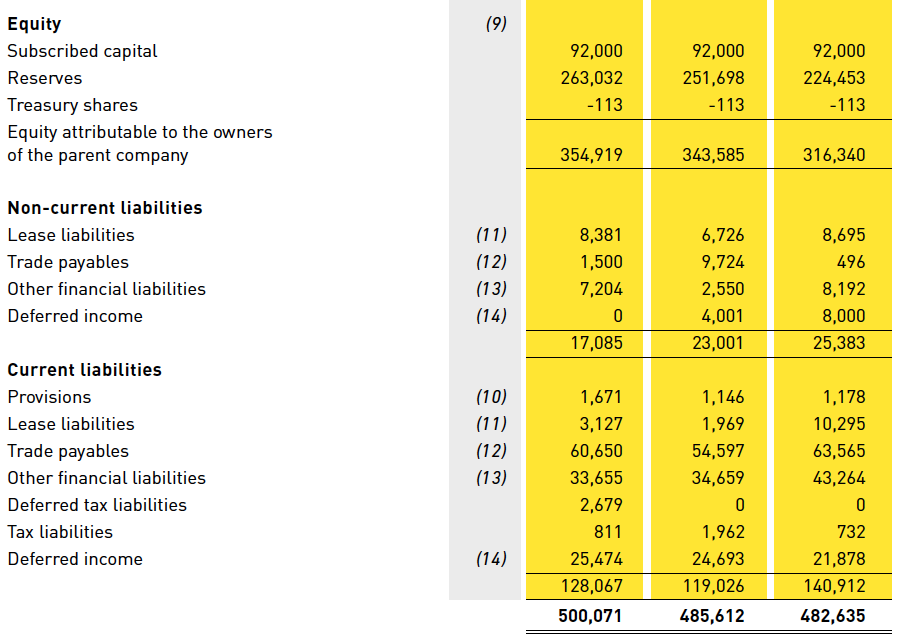
\includegraphics[width=.45\textwidth]{img/SP_passivo_dor.png} \label{sp_passivo_dor}}
            \caption{Stato Patrimoniale Borussia Dortmund al 30 Giungno 2019}
            \label{sp_dor}  
        \end{figure}
        \begin{equation}
                \text{Margine di Tesoreria} = 123.787.000-128.067.000 = \mathbf{-4.280.000\mbox{\euro}}
            \label{eqn: marg_teso_dor}
        \end{equation}
        \begin{equation}
                \text{Indice di liquidit\'a primaria} = \frac{123.787.000}{128.067.000} = \mathbf{96,65\%}
            \label{eqn: ind_liq_dor}
        \end{equation}
       Per la prima volta troviamo una situazione positiva per la posizione di liquidit\'a: il margine di tesoreria \'e si negativo, ma di solo
       4mln€ e l'indice di liquidit\'a spiega come le passivit\'a a breve siano coperte per il 96\% da mezzi liquidi e quindi subito disponbili,
       rendendo il Borussia una societ\'a che nel complesso puo\'o far fronte completamente ai debiti nel breve termine.
    \item Analisi della solidit\'a:\newline
        \begin{equation}
            \text{Grado di Indipendenza Finanziaria} = \frac{354.919.000}{500.071.000} = \mathbf{70,97\%}
        \label{eqn: indeb_dor}
        \end{equation}
        \begin{equation}
            \text{Margine di Struttura} = 354.919.000-348.085.000 = \mathbf{6.834.000\mbox{\euro}}
            \label{eqn: marg_strutt_dor}
        \end{equation}
        Anche in questo caso troviamo una situazione molto positiva: il grado di indipendenza finanziaria mostra che tramite il patrimonio
        netto la societ\'a riesce ad affrontare il 70\% del valore delle passivit\'a, a riprova della oculata gestione economica tedesca.
        Anche il margine di struttura non \'e da meno dato che per la prima volta troviamo un valore positivo, a dimostrazione tramite i mezzi
        propri sono pefettamente in grado di far fronte a tutte immobilizzazioni.  \newline
    \item Analisi della Redditivit\'a:\newline
        \begin{equation}
            \text{ROI} = \frac{23.501.000}{500.071.000} = \mathbf{4,6\%}
        \label{eqn: roi_dor}
        \end{equation}
        \begin{equation}
            \text{ROE} = \frac{17.391.000}{354.919.000} = \mathbf{4,8\%}
        \label{eqn: roe_dor}
        \end{equation}
        Anche in quest'ultimo caso i risultati sono incoraggianti: il ROI \'e positivo grazie ovviamente al fatto che \'e presente un 
        risultato d'esercizio positivo (anche se in diminuzione rispetto all'anno precedente) e con un valore di 4,6\% evidenzia la capacit\'a
        della societ\'a di far fruttare gli investimenti effettuati; il ROE, anch'esso positivo evidenzia invece come gli investimenti fatti con 
        capitale proprio stia andando nella giusta direzione.
\end{enumerate}
\subsection{Barcellona}
Quarto club soggetto dell'analisi \'e il Barcellona, una delle squadre pi\'u titolate e tifate al mondo la quale vanta un \emph{palmares} di:
26 campionati, 31 Coppe di Spagna, 2 Coppe della Liga, 13 Supercoppe di Spagna e 3 Coppe de Oro Argentina\footnote{https://it.wikipedia.org/wiki/Futbol\_Club\_Barcelona}.
\'E l'unica squadra, insieme al Bayern Monaco, ad aver conquistato il \emph{sextuple} riuscendo a vincere tutte le 6 competizioni nazionali e
internazionali disponibili durante l'anno. Insieme al Real Madrid formano una delle rivalit\'a pi\'u antiche e accese della storia Europea, 
possedendo anche un nome unico per la partita con quest'ultima: \emph{El Clasico}.\newpage
\begin{enumerate}
    \item Analisi dei Ricavi:\newline
        \begin{figure}
            \centering
            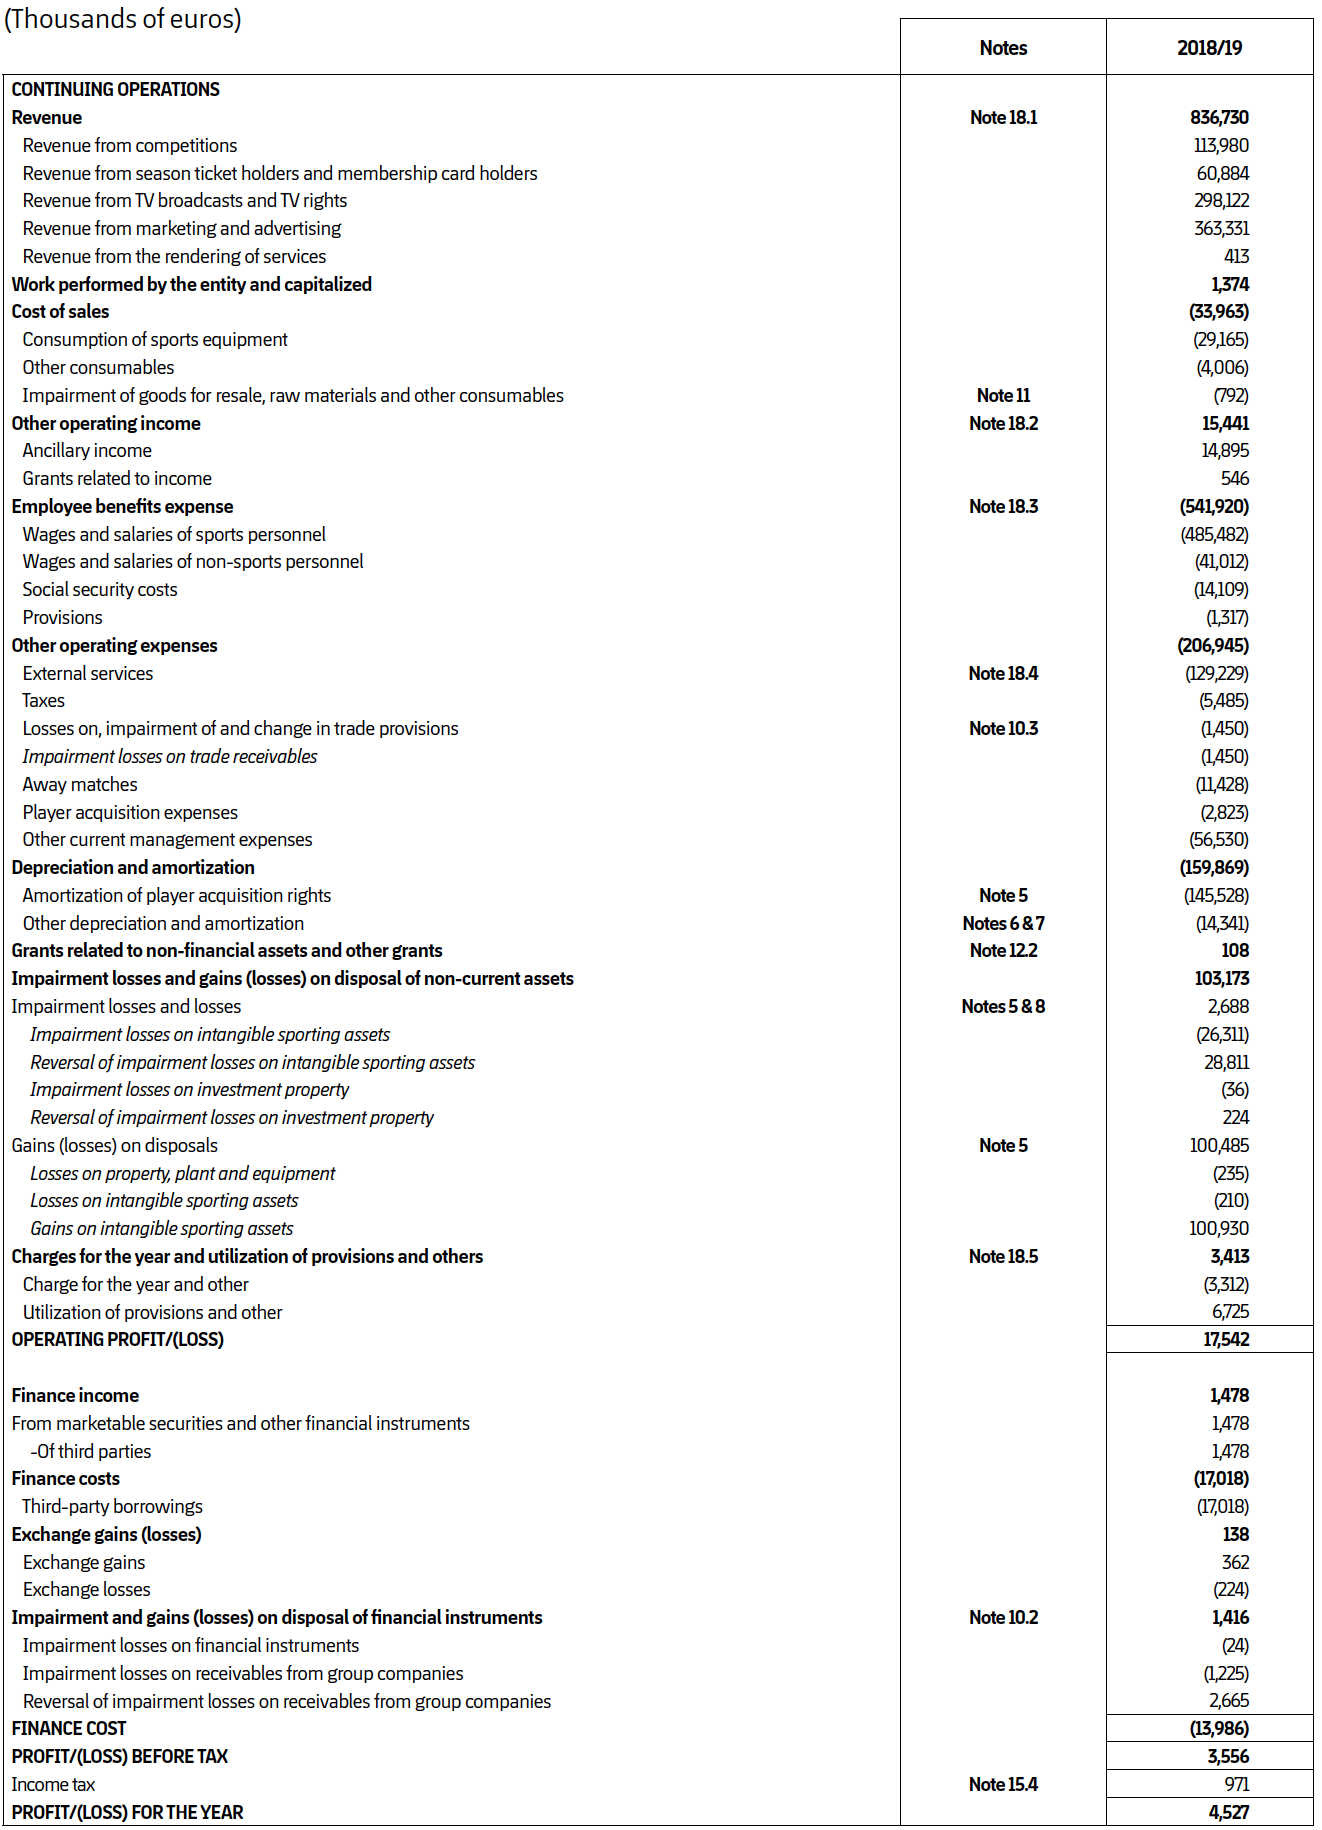
\includegraphics[scale=.5]{img/CE_barca.png}
            \caption{Conto Economico Barcellona al 30 Giugno 2019}
            \label{ce_barca}
        \end{figure}\newline
        \begin{equation}
            \frac{\text{Ricavi da gare}}{\text{Totale Ricavi}} = \frac{170.864.000}{837.730.000} = \mathbf{20,8\%}
            \label{eqn: gare_barca}
        \end{equation}
        \begin{equation}
            \frac{\text{Diritti TV}}{\text{Totale Ricavi}} = \frac{298.122.000}{837.730.000} = \mathbf{35,62\%}
            \label{eqn: tv_barca}
        \end{equation}
        \begin{equation}
            \frac{\text{Ricavi commerciali}}{\text{Totale Ricavi}} = \frac{363.331.000}{837.730.000} = \mathbf{43,42\%}
            \label{eqn: commerc_barca}
        \end{equation}
        La premessa fatta poco prima si riconferma in questa sezione: la parte dei ricavi commerciali copre quasi la met\'a dei ricavi totale,
        a riprova di quanto sia famosa la societ\'a in tutto il mondo; anche i diritti tv prendono una bella fetta del totale dato che
        la Liga Santander \'e molto seguita in tutta Europa ma anche in altri paesi di lingua Spagnola; i ricavi da gare hanno anch'essi 
        una discreta importanza a dimostrazione di come il calcio in Spagna sia molto seguito.
    \item Analisi della liquidit\'a:\newline
        \begin{figure}
            \centering
            \subfloat[][Stato Patrimoniale attivo al 30 Giugno 2019]
            {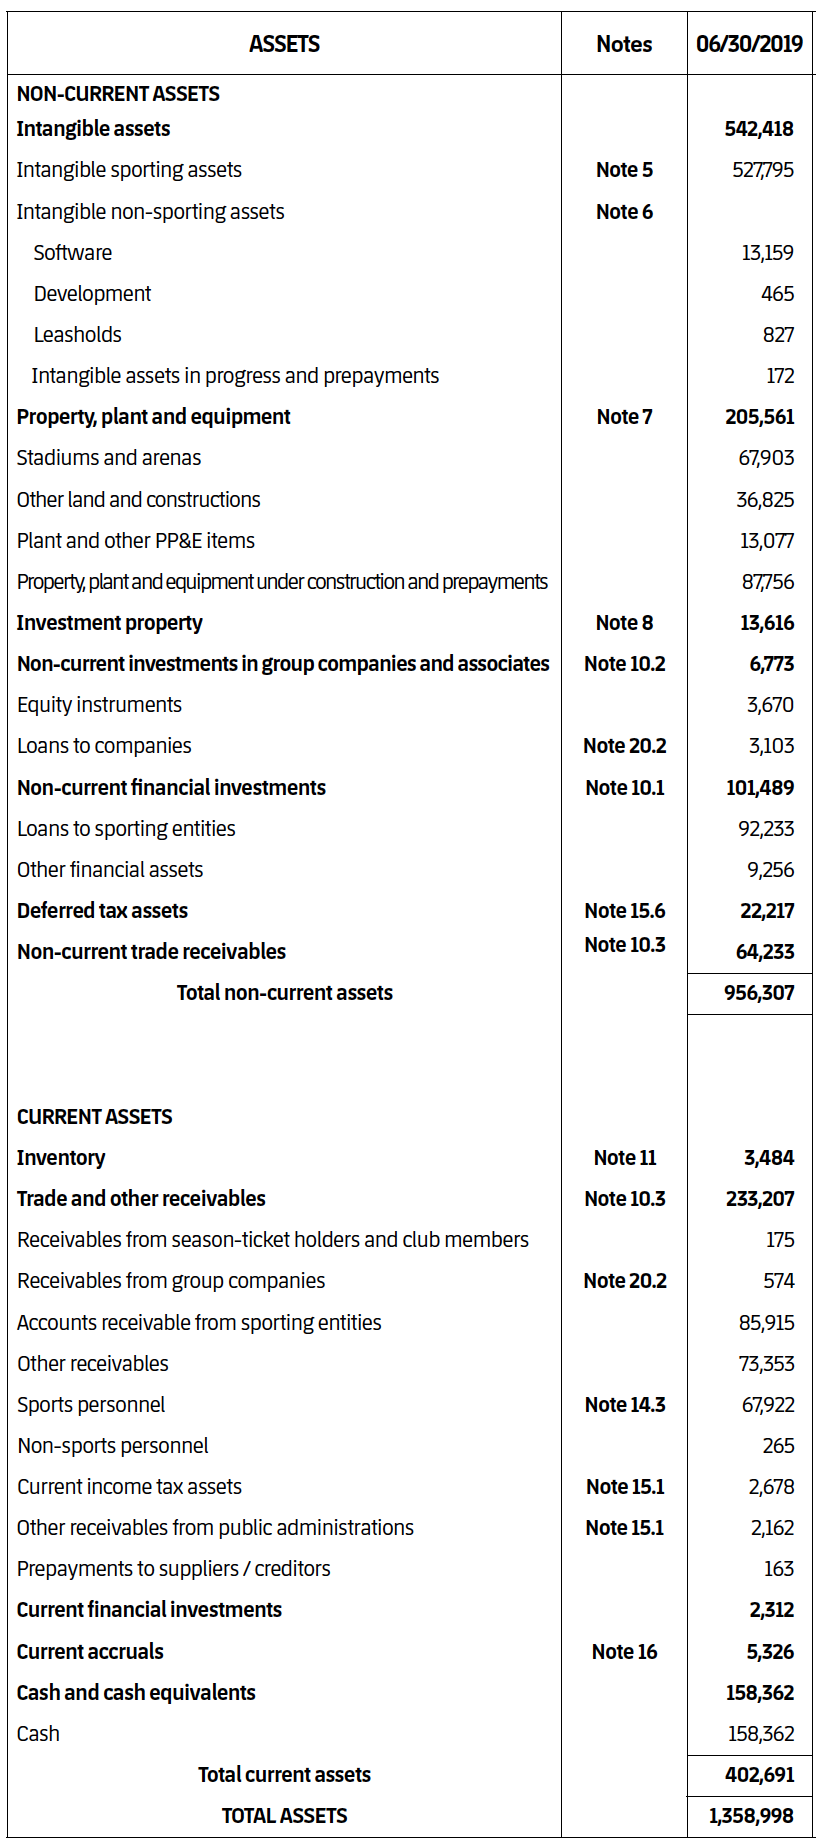
\includegraphics[width=.45\textwidth]{img/SP_attivo_barca.png} \label{sp_attivo_barca}} \quad
            \subfloat[][Stato Patrimoniale passivo al 30 Giugno 2019]
            {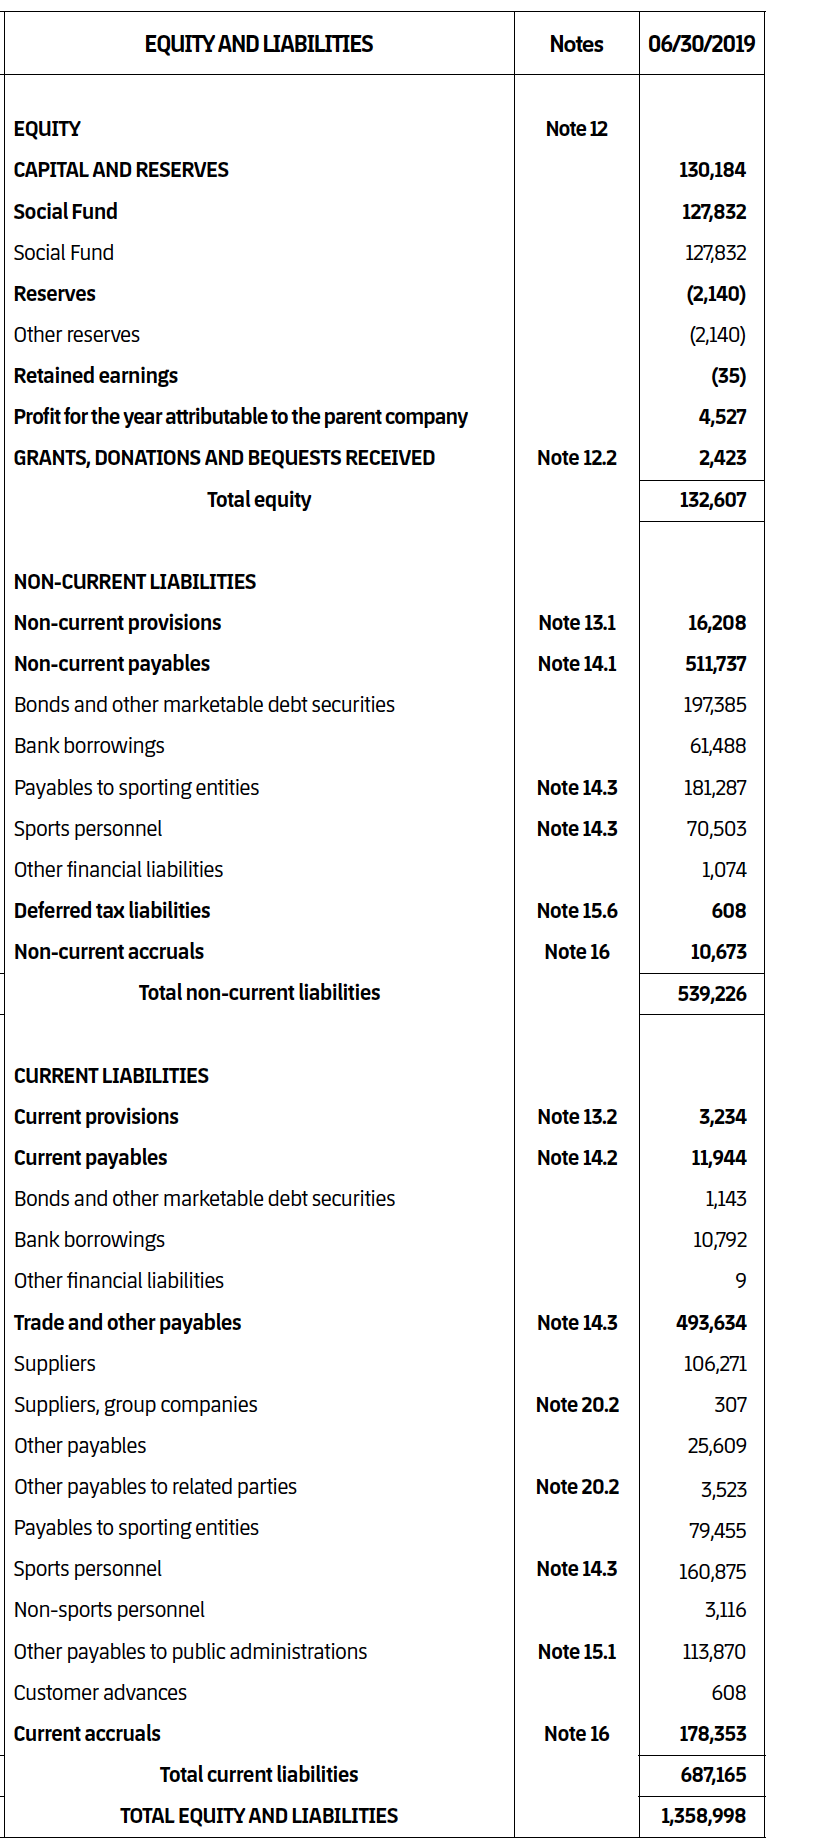
\includegraphics[width=.45\textwidth]{img/SP_passivo_barca.png} \label{sp_passivo_barca}}
            \caption{Stato Patrimoniale Barcellona al 30 Giungno 2019}
            \label{sp_barca}  
        \end{figure}
        \begin{equation}
                \text{Margine di Tesoreria} = 399.207.000-687.165.000 = \mathbf{-287.958.000\mbox{\euro}}
            \label{eqn: marg_teso_barca}
        \end{equation}
        \begin{equation}
                \text{Indice di liquidit\'a primaria} = \frac{399.207.000}{687.165.000} = \mathbf{58,09\%}
            \label{eqn: ind_liq_barca}
        \end{equation}
       Dopo una prima analisi positiva torniamo ora ad affrontare una sezione pi\'u complessa: l'indice di liquidit\'a primario
       che esprime in percentuale il margine di tesoreria mostra come circa la met\'a delle passivit\'a a breve termine sia scoperta dalle
       liquidit\'a disponbili, andando a creare un problema nel caso serva ripagare le passivit\'a a breve termine.
    \item Analisi della solidit\'a:\newline
        \begin{equation}
            \text{Grado di Indipendenza Finanziaria} = \frac{132.607.000}{1.358.998.000} = \mathbf{9,7\%}
        \label{eqn: indeb_barca}
        \end{equation}
        \begin{equation}
            \text{Margine di Struttura} = 132.607.000-747.979.000 = \mathbf{-615.372.000\mbox{\euro}}
        \label{eqn: marg_strutt_barca}
        \end{equation}
        Anche la solidit\'a della societ\'a non produce risultati molto soddisfacenti: il patrimonio netto non finanzia neanche il 10\% 
        delle passivit\'a totali, mentre le immobilizzazioni risultano "scoperte" per pi\'u di 600mln€. Questi risultati evidenziano come
        la societ\'a faccia uso quasi nella totalit\'a al capitale di debito.\newpage
    \item Analisi della Redditivit\'a:\newline
        \begin{equation}
            \text{ROI} = \frac{17.542.000}{1.358.988.000} = \mathbf{1,29\%}
        \label{eqn: roi_barca}
        \end{equation}
        \begin{equation}
            \text{ROE} = \frac{23.501.000}{354.919.000} = \mathbf{6,62\%}
        \label{eqn: roe_barca}
        \end{equation}
        Confrontando invece voci economiche e patrimoniali i risultati cambiano: il risultato operativo rimane positivo grazie ai risultati sportivi
        raggiunti e ad alcune operazioni di mercato che hanno alleggerito in modo minimo le casse del club, rendendo quindi il ROI positivo 
        ma molto vicino allo 0; il ROE invece ha un valore positivo e maggiore di 0 andando quindi a mostrare come, seppur pochi, investimenti 
        fatti con i mezzi propri siano buoni.
\end{enumerate}
\subsection{Manchester City}
Come ultimo club di questa prima parte della trattazione andremo a vedere il Manchester City, squadra di grande peso in Inghilterra anche se,
come \'e accaduto con il Paris Saint Germain, solo grazie all'acquisto del club da parte di sceicchi in grado di effettuare grandi investimenti 
senza troppe preoccupazioni sul ritorno. Dalla sua fondazione, nel 1894, fino al 2008 (anno dell'approdo degli sceicchi in Premier League) i \emph{Citizens} "ventavano"
un bacheca contenente: 2 campionati inglesi, 4 coppe d'inghilterra, 2 coppe di lega inglesi, 3 Community Shield e 1 Coppa delle Coppe. 
In soli 10 anni invece \'e riuscita a conquistare: 4 campionati inglesi, 2 coppe d'inghilterra, 4 coppe di lega e 3 Community Shield\footnote{https://it.wikipedia.org/wiki/Manchester\_City\_Football\_Club\#Palmar\%C3\%A8s}.\newpage
\begin{enumerate}
    \item Analisi dei Ricavi:\newline
        \begin{figure}
            \centering
            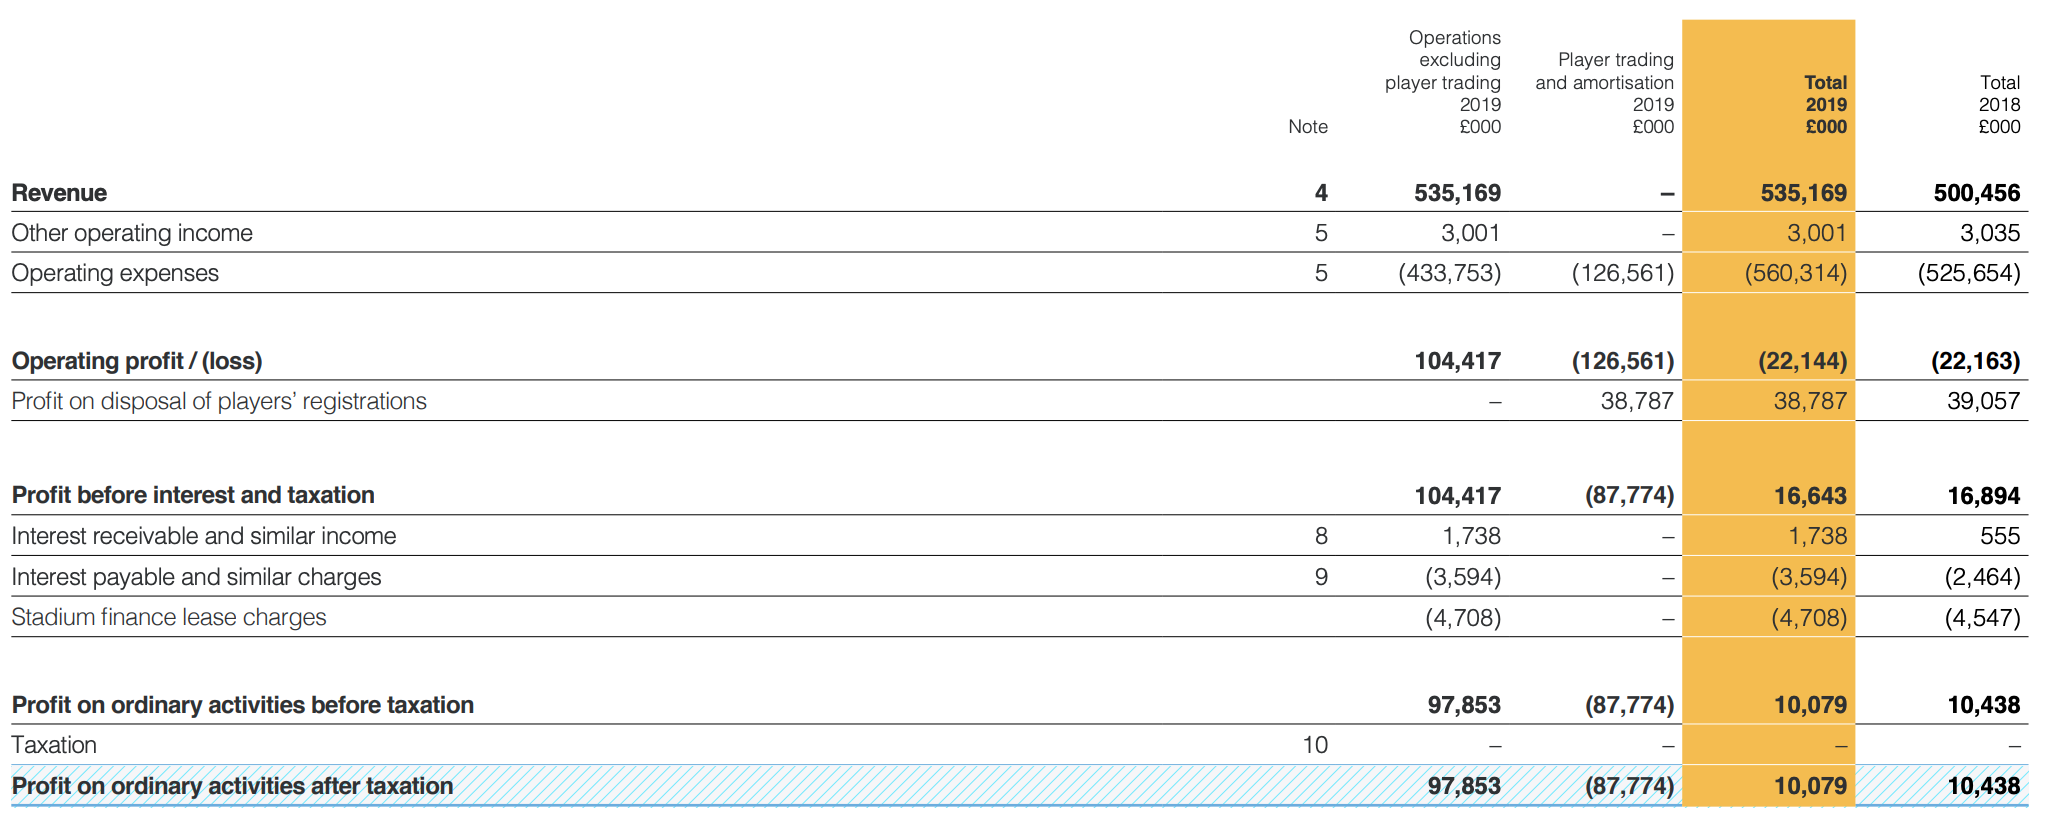
\includegraphics[scale=.4]{img/CE_city.png}
            \caption{Conto Economico Manchester City al 30 Giugno 2019}
            \label{ce_city}
        \end{figure}\newline
        \begin{equation}
            \frac{\text{Ricavi da gare}}{\text{Totale Ricavi}} = \frac{55.007.000}{535.169.000} = \mathbf{10,27\%}
            \label{eqn: gare_city}
        \end{equation}
        \begin{equation}
            \frac{\text{Diritti TV}}{\text{Totale Ricavi}} = \frac{253.176.000}{535.169.000} = \mathbf{47,30\%}
            \label{eqn: tv_city}
        \end{equation}
        \begin{equation}
            \frac{\text{Ricavi commerciali}}{\text{Totale Ricavi}} = \frac{228.833.000}{535.169.000} = \mathbf{42,75\%}
            \label{eqn: commerc_city}
        \end{equation}
        Dal punto di vista dei ricavi, la societ\'a pu\'o giovare di due grandi propriet\'a del calcio inglese: essere uno dei campionati
        pi\'u seguiti al mondo e di conseguenza avere fan in giro per il mondo che contribuiscono all'acquisto dei prodotti de club. Per questo 
        motivo i ricavi commerciali e quelli da diritti tv sono molto elevati e compongono la quota maggiore sul totale. I ricavi da gare
        rimangono in percentuale stabili.\newpage
    \item Analisi della liquidit\'a:\newline
        \begin{figure}
            \centering
            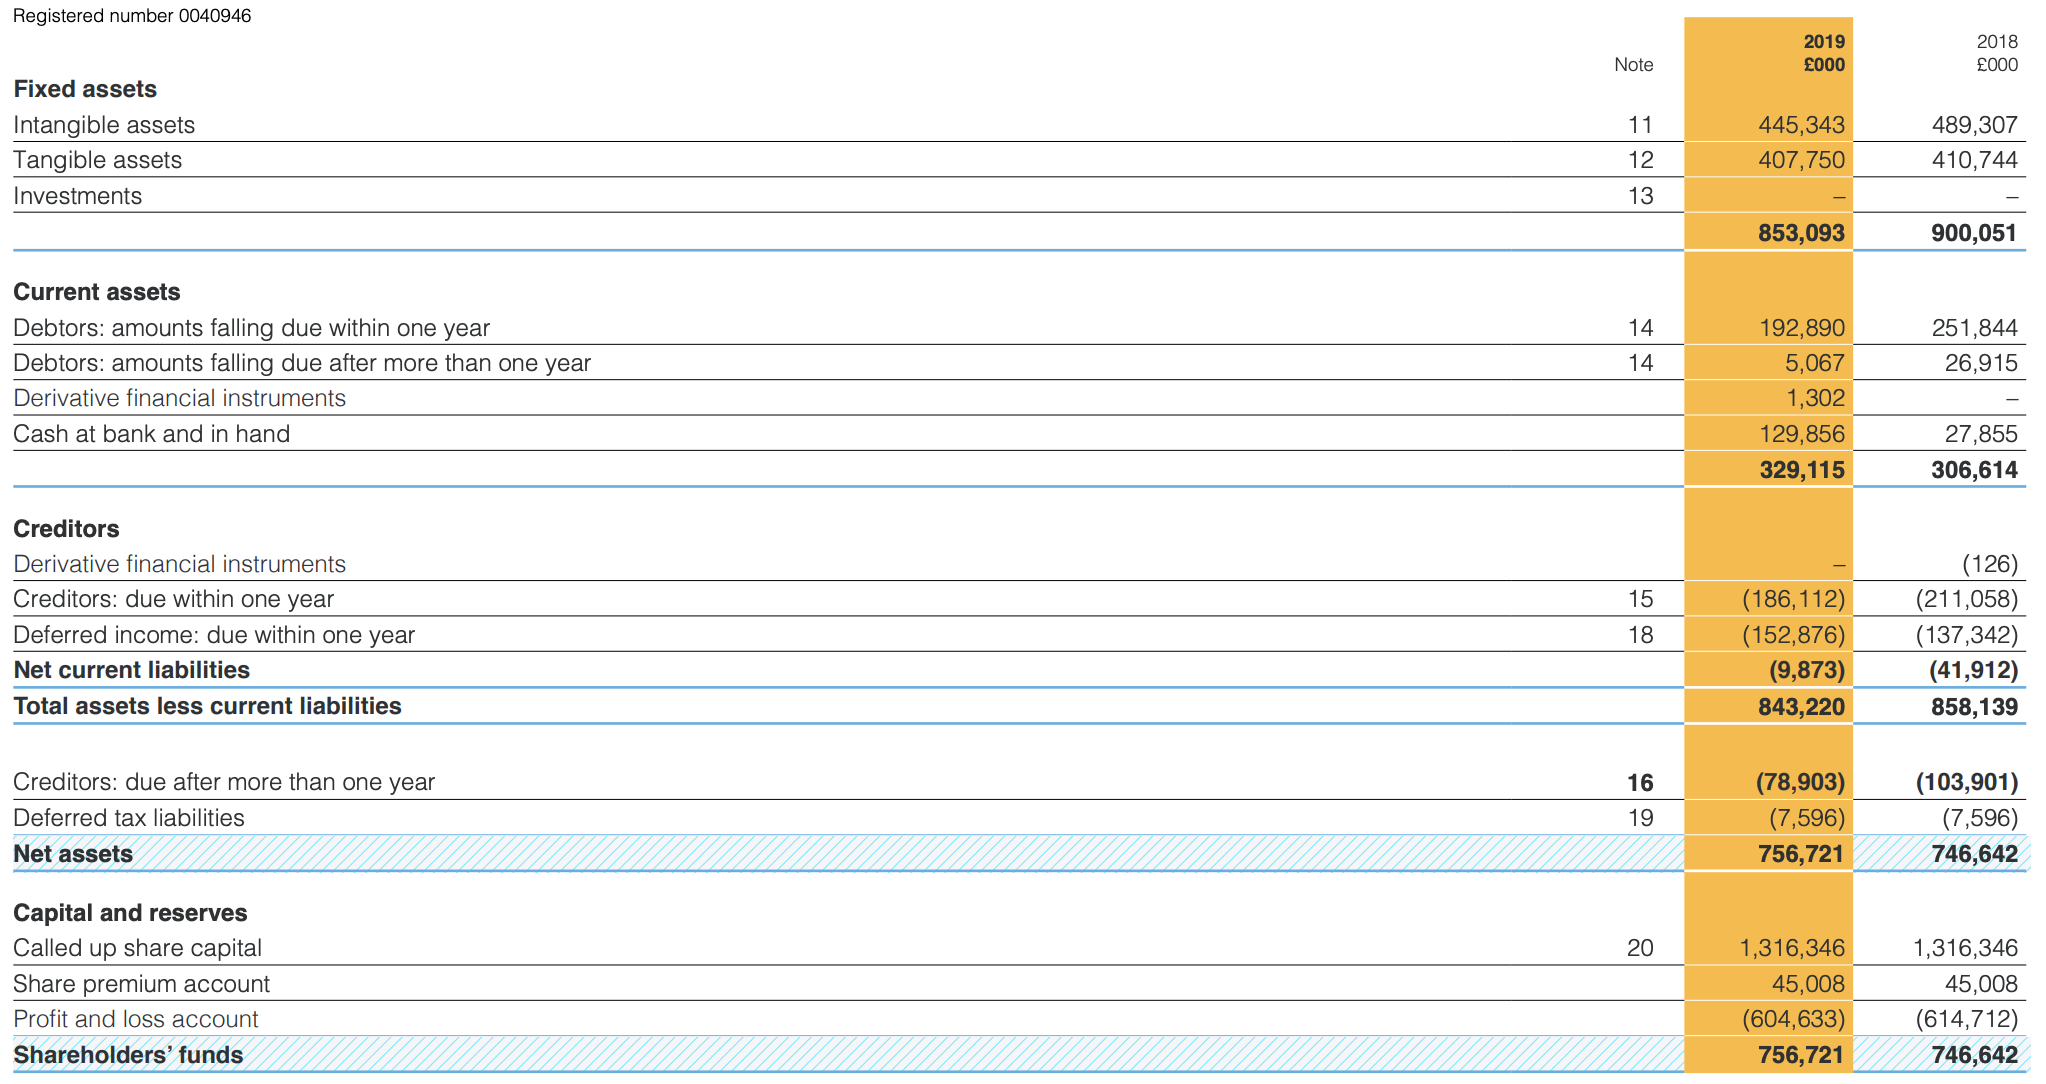
\includegraphics[scale=.4]{img/SP_city.png}
            \caption{Stato Patrimoniale Manchester City al 30 Giugno 2019}
            \label{sp_city}
        \end{figure}\newline
        \begin{equation}
                \text{Margine di Tesoreria} = 129.856.999 - 843.220.000 = \mathbf{-713.364.000\pounds}
            \label{eqn: marg_teso_city}
        \end{equation}
        \begin{equation}
                \text{Indice di liquidit\'a primaria} = \frac{129.856.999}{843.220.000} = \mathbf{15,40\%}
            \label{eqn: ind_liq_city}
        \end{equation}
        Anche in questo caso troviamo uno scenario simile a quello del Barcellona. Se da un lato i ricavi possono avere il loro significato 
        mostrando come una societ\'a produca effettivamente risultati nel breve periodo, dal punto di vista patrimoniale non si pu\'o dire 
        lo stesso: le passivit\'a a breve termine sono scoperte per quasi la totalit\'a del loro valore, solo il 15\% potr\'a essere 
        coperto con denaro liquido e disponibile sin da subito.
    \item Analisi della solidit\'a:\newline
        \begin{equation}
            \text{Grado di Indipendenza Finanziaria} = \frac{756.721.000}{1.182.208.000} = \mathbf{64,00\%}
        \label{eqn: indeb_city}
        \end{equation}
        \begin{equation}
            \text{Margine di Struttura} = 756.721.000 - 853.093.000 = \mathbf{-96.372.000\pounds}
            \label{eqn: marg_strutt_city}
        \end{equation}
        Per quanto riguarda la solidit\'a troviamo un grado di indipendenza finanziaria positivo, stando a significare un buon grado di autonomia
        rispetto ai finanziatori esterni. Il margine di struttura evidenzia come le immobilizzazioni (materiali, immateriali e finanziarie) non 
        siano per\'o completamente coperte dal Patrimonio Netto, con uno scoperto comunque accettabile pari a meno di 100mln£.
    \item Analisi della Redditivit\'a:\newline
        \begin{equation}
            \text{ROI} = \frac{-22.154.000}{1.182.208.000} = \mathbf{-1,81\%}
        \label{eqn: roi_city}
        \end{equation}
        \begin{equation}
            \text{ROE} = \frac{10.079.000}{756.721.000} = \mathbf{1,33\%}
        \label{eqn: roe_city}
        \end{equation}
        Anche nell'ultima parte di analisi i risultati non sono molto consistenti. Se si considera il risultato operativo esclusi 
        i ricavi dallo scambio dei giocatori, da un profitto si arriva ad una perdita, a dimostrazione di come sia importante e pesante
        il business dei calciatori e dei loro cartellini. Il ROE, invece, che considera il risultato netto, si "salva" grazie ai profitti
        sulla cessione di registrazione dei calciatori che elimina la perdita generata con la sola sottrazioen di ricavi e costi.
\end{enumerate}
\chapter{Fair Play Finanziario}
\section{Dalla nascita alle ultime riforme}
Il \textbf{Fair Play Finanziario} \'e un insieme di norme dettate dalla UEFA, che cercano di porre rimedio alla molto negativa situazione econmico-
finanziaria del sistema calcio, generatasi a partire dall'inizio degli anni 90 e che ancora oggi, come abbiamo avuto modo di notare, non 
\'e stata del tutto risolta.
Questa nuova idea di porre dei "paletti" alle societ\'a durante la loro attivit\'a e relativamente alla redazione del bilancio, \'e
nata in seguito ad una indagine condotta dalla UEFA nel 2010, su pi\'u di 600 Club in Europa. Questa ricerca mostrava come pi\'u della met\'a
dei Club coinvolti, e di questa met\'a la maggior parte erano di grandi dimensioni, presentava ingenti perdite d'esercizio. Da quel momento
la Federazione decise che si dovesse intevenire in qualche modo, specialmente su 3 macro-aree:
\begin{enumerate}
    \item \textbf{Debiti scaduti non pagati}: la maggior parte delle societ\'a presentavano una posizione debitoria nei confronti
    di dipendenti ed Erario non molto positiva.
    \item \textbf{Incidenza del costo del lavoro sul totale dei ricavi}: uno dei problemi principali delle societ\'a di calcio odierne, dato
    dalla sempre maggiore forza contrattuale esercitata dai calciatori e i loro procuratori.
    \item \textbf{Rapporto squilibrato tra ricavi e costi}: derivazione del punto precedente, ed in aggiunta, dato lo scarso interesse verso
    accordi commerciali i ricavi non potranno mai riuscire a coprire i costi.
\end{enumerate}
In seguito ad aver riconosciuto le aree in cui fosse necessario migliorare \'e stata presa la decisione di redigere, il 27 Maggio 2010, la 
\textbf{\emph{Uefa Club Licensing and Financial Fair Play Regulation}} in accordo con tutte le societ\'a europee.
Il documento prevede degli obiettivi di carattere sociale e di crescita collettiva ma anche, ovviamente, economico\footnote{UEFA: https://documents.uefa.com/v/u/MFxeqLNKelkYyh5JSafuhg}:
\begin{enumerate}[(a)]
    \item Promuovere ulteriormente e migliorare continuamente il livello di tutti gli aspetti del
    del calcio in Europa e a dare costante priorità alla formazione e alla cura dei
    giovani giocatori in ogni club; 
    \item Assicurare che i club abbiano un livello adeguato di gestione e organizzazione;
    \item Adattare le infrastrutture sportive dei club per fornire a giocatori, spettatori e rappresentanti dei media
    strutture adeguate, ben attrezzate e sicure;
    \item Proteggere l'integrità e il regolare svolgimento delle competizioni UEFA per club;
    \item Permettere lo sviluppo del benchmarking per i club in termini di criteri finanziari, sportivi, legali,
    legali, personali, amministrativi e infrastrutturali in tutta Europa.
    \item Migliorare la capacità economica e finanziaria dei club, aumentando la loro
    trasparenza e credibilità;
    \item Dare l'importanza necessaria alla protezione dei creditori e garantire
    che i club saldino puntualmente i loro debiti con i dipendenti, le autorità sociali/fiscali e gli altri
    club in modo puntuale;
    \item Introdurre più disciplina e razionalità nelle finanze del calcio dei club;
    \item Incoraggiare i club ad operare sulla base delle proprie entrate;
    \item incoraggiare la spesa responsabile per il beneficio a lungo termine del calcio;
    \item Proteggere la redditività e la sostenibilità a lungo termine del calcio europeo per club.
\end{enumerate}
Entrando più nello specifico, la UEFA ho dovuto introdurre alcune misure specifiche per fare in modo che i club entrassero in questa nuova 
mentalit\'a di \emph{spendere solo i soldi che si hanno}, puntando quindi ad un obiettivo di \textbf{pareggio di bilancio} e \textbf{
gestione dei costi}. Come abbiamo avuto modo di vedere nel primo capitolo, per\'o, i club con molte disponibilit\'a economiche non hanno
tenuto a mente questa regola, andando a creare situazione di incertezza molto forte, causata da una spesa senza controllo che non va' a 
pareggiare i ricavi generati. Proprio per quanto riguarda i ricavi, dal momento in cui il Fair Play Finanziario \'e entrato in vigore, le 
societ\'a hanno dovuto porre una maggiore attenzione all'aspetto delle entrate: essendo l'unico modo per creare una situazione di 
equilibrio economico esse si sono dovute ridimensionare, ponendo maggior impegno su di esse. Se si osserva infatti il totale dei ricavi
generati dalle principali squadre europee dal 2010 ad oggi (2019) si pu\'o osservare quanto segue:
\begin{figure}
    \centering
    \subfloat[][Ricavi all'anno 2010]
    {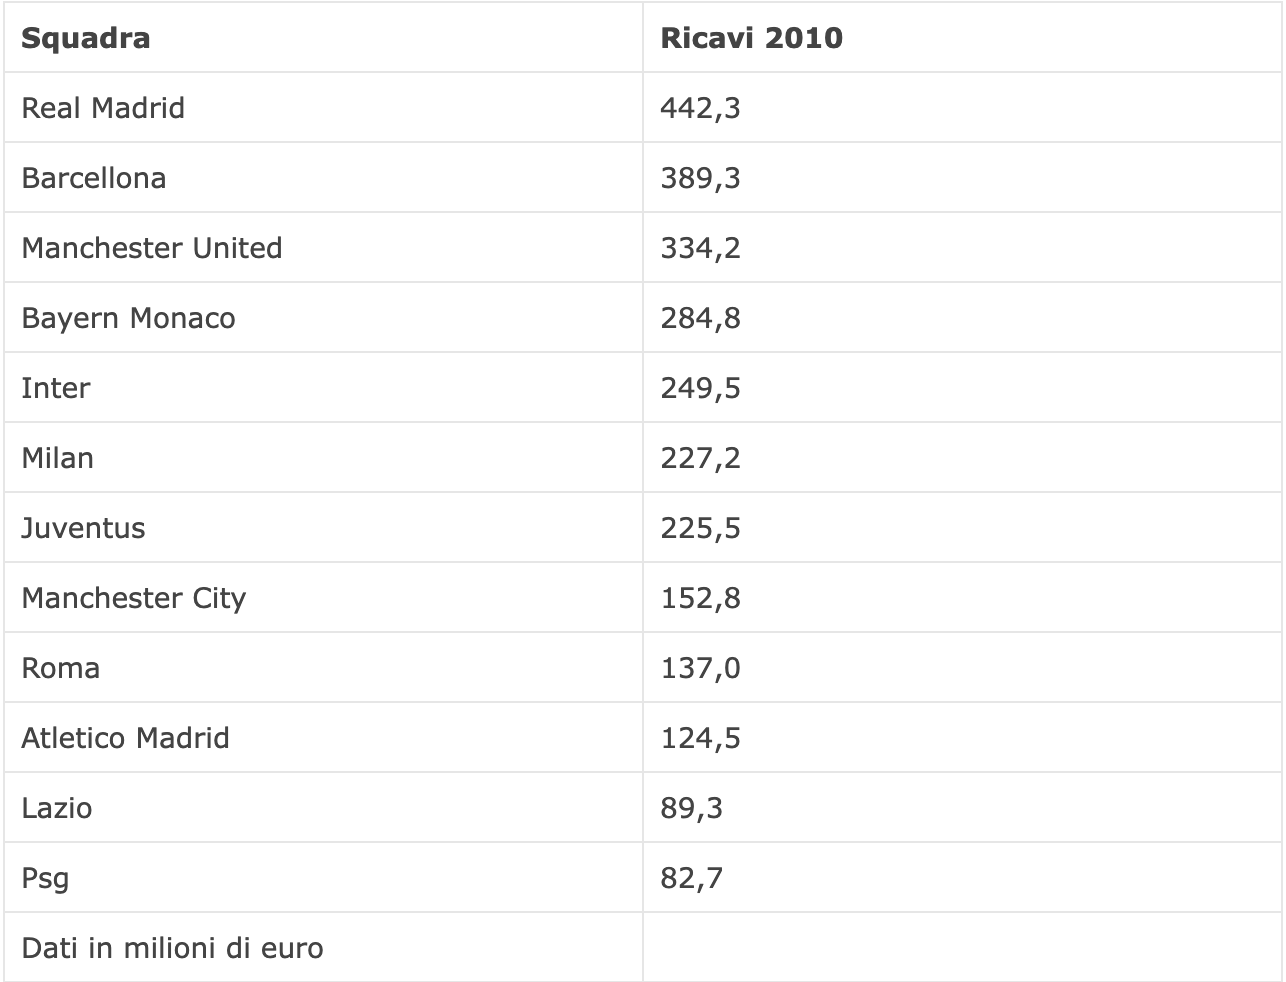
\includegraphics[width=.35\textwidth]{img/ricavi_2010.png} \label{ricavi_2010}} \quad
    \subfloat[][Ricavi all'anno 2019]
    {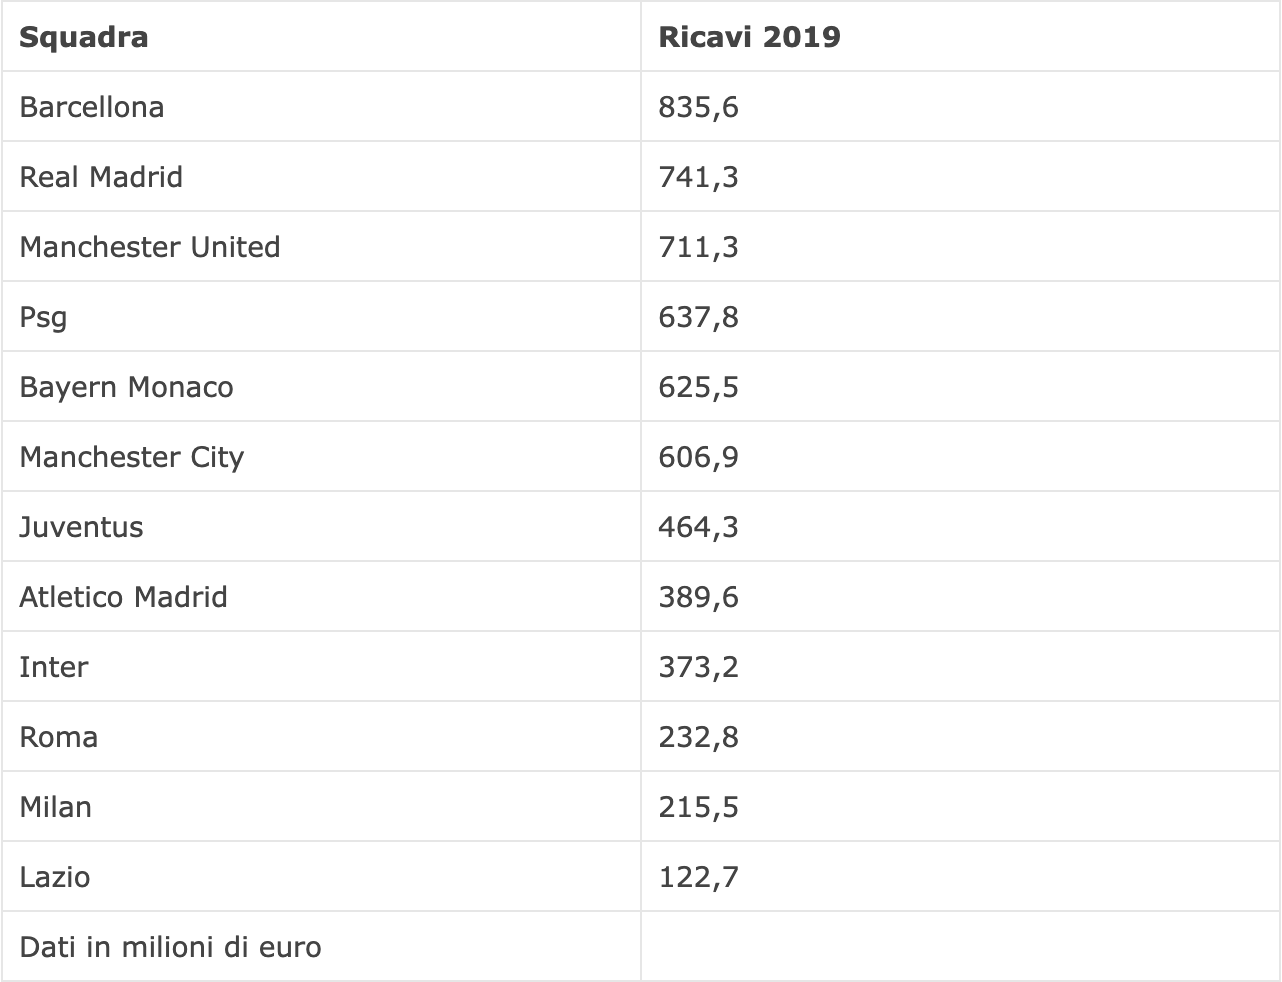
\includegraphics[width=.35\textwidth]{img/ricavi_2019.png} \label{ricavi_2019}}
    \caption{Comparazione ricavi 2010-2019}
    \label{comp_ricavi_10_19}  
\end{figure}
Come mostra la figura \ref{comp_ricavi_10_19}\footnote{https://www.calcioefinanza.it/2019/12/30/classifica-ricavi-squadre-decennio-juve-inter-milan/}
in seguito all'approvazione del \emph{FFP} i principali club europei hanno captato la necessit\'a di modificare qualcosa nel loro core business,
sopratutto quanro riguarda la voce dei ricavi da gare, ricavi da diritti televisivi e ricavi commerciali\footnote{Analisi presente nel Capitolo Uno}.
L'incremento maggiore \'e stato, quasi ovviamente si potrebbe dire, quello del Paris Saint Germain che ha registrato un +671.2\%, certamente
grazie all'approdo degli sceicchi alla dirigenza del Club; nelle posizione successive troviamo i principali Club di Germania, Inghilterra e Spagna
con incrementi superiori al 100\%; infine solo nelle ultime posizioni troviamo le societ\'a Italiane, capitanate dalla Juventus con anch'essa un aumento 
poco superiore al 100\%. Per ultima, la societ\'a AC Milan che vede addirittura un decremento rispetto al 2010, specificatamente del 5.1\%
questo a causa di un periodo buio in quanto a risultati sportivi, che hanno portato meno tifosi allo stadio ma sopratutto meno incassi 
da diritti televisivi.\newline
Questo rinnovato interesse delle societ\'a rispetto a questi aspetti che coinvolgono in misura considerevole il consumatore finale, ha fatto
si che quest'ultimo riuscisse a giovarne si tutte queste nuove attenzioni, andando per esempio a considerare la partita allo stadio come
un momento da vivere a 360 gradi che ti deve coinvolgere dal momento in cui entri al momento in cui esci.\newline
Tornando ad aspetti maggiormente economici, uno dei pilastri principali su cui i basa il \emph{Fair Play Finanziario} \'e la \emph{\textbf{Break-even Rule}}.
Essa viene articolata a partire dall'articolo 57 del documento e specifica come le squadre che vogliano partecipare a competizioni UEFA debbano
rispettare il pareggio di bilancio e altre regolamentazioni di tipo economico-finanziarie. Il rispetto di queste regole per\'o si basa su 
un \emph{monitoring period}, cio\'e un periodo di monitoraggio nel quale la Federazione effettua dei controlli per poter arrivare in seguito 
ad un giudizio ponderato e corretto. Il periodo di monitoraggio si basa sui 2 esercizi precedenti a quello preso in considerazione pi\'u quello attuale,
e al termine dell'analisi non si deve aver infranto nessuno dei punti presenti all'Articolo 62 parte 3, al cui interno 
\'e compresa anche la \emph{Break-Even Rule}. Vi sono per\'o delle condizioni in cui \'e possibile infrangere uno dei punti della parte 3 
ed essere ugualmente in grado di soddisfare i requisiti per ottenere la licenza UEFA:
\begin{enumerate}
    \item Il club che presenta la richiesta per la licenza deve aver conseguito un utile nei tre periodi precedenti all'analisi;
    \item Il club che richiede la licenza presenta una perdita ma all'interno del margine delineato all'interno dell'art. 61 parte 2\footnote{Massimo 5 milioni di euro oppure 30 milioni in caso la perdita sia contenuta con contributi delle partecipate e/o parti correlate}
\end{enumerate}
Per poter spiegare in modo pi\'u concreto il significato della \emph{Break-Even Rule} \'e necessario capire come arrivare al punto di pareggio.
In Economia, il punto di pareggio (\emph{Break-Even Point}) viene identificato tramite la quantit\'a da vendere necessaria a coprire i costi 
sostenuti per la produzione, per poter terminare il periodo senza perdite o profitti. Anche in questo caso la regola applicata \'e la stessa,
ma per la UEFA \'e necessario considerare solo i \textbf{Ricavi Rilevanti} e i \textbf{Costi Rilevanti}.
\newpage
\begin{table}
    \begin{tabularx}{\textwidth}{XX}
        \toprule
        \textbf{Ricavi Rilevanti} & \textbf{Costi Rilevanti} \\
        \midrule
        Ricavi da gare & Costi dei materiali (voce che comprende tutti gli aspetti dell'attivit\'a sportiva) \\
        \midrule
        Ricavi da diritti TV & Costo del personale \\
        \midrule
        Sponsor e pubblicit\'a & Costi per organizzazione gare e affitto impianti sportivi \\
        \midrule
        Ricavi commerciali & Ammortamenti e svalutazioni relative ai calciatori \\
        \midrule
        Ricavi da cessione calciatori & Gli oneri finanziari e dividendi \\
        \midrule
        Ricavi da cessione di immobilizzazioni & \\
        \bottomrule
    \end{tabularx}
    \caption{Tabella Costi e Ricavi Rilevanti}
    \label{tabella_ric_costi_ril}
\end{table} 
Tramite la tabella \ref{tabella_ric_costi_ril} \'e possibile capire in modo pi\'u immediato cosa racchiudono queste due voci. La voce principale 
che non viene considerata per il calcolo del \emph{Break-Even} \'e quella realtiva al settore giovanile, che essendo eslusa da queste regole
permette ai club di investire senza dover pensare ad alcun tipo di regola economico-finanziaria, permettendogli di generare un potenziale ritorno
elevatissimo. L'esempio forse pi\'u lampante di societ\'a che ha accolto in modo positivo questa norma \'e l'Ajax, una delle pi\'u famose
squadre olandesi e famosa in tutto il mondo perch\'e capace ogni anno di produrre talenti dal settore giovanile per poi venderli successivamente
producendo plusvalenze notevolissime.\newline
In conclusione, quindi, i criteri di base per il rispetto del \emph{Fair Play Finanziario} non sono fondamentalmente complicati, ma, come 
si potr\'a vedere successivamente non tutte le societ\'a sono state intenzionate a rispettarlo.
\subsection{Le riforme del 2014 e del 2015}
\end{interlinea}
\end{document}

